\documentclass[]{article}
\usepackage{lmodern}
\usepackage[compact]{titlesec}
\usepackage{amssymb,amsmath}
\usepackage{ifxetex,ifluatex}
\usepackage{fixltx2e} % provides \textsubscript
\ifnum 0\ifxetex 1\fi\ifluatex 1\fi=0 % if pdftex
  \usepackage[T1]{fontenc}
  \usepackage[utf8]{inputenc}
\else % if luatex or xelatex
  \ifxetex
    \usepackage{mathspec}
  \else
    \usepackage{fontspec}
  \fi
  \defaultfontfeatures{Ligatures=TeX,Scale=MatchLowercase}
\fi
% use upquote if available, for straight quotes in verbatim environments
\IfFileExists{upquote.sty}{\usepackage{upquote}}{}
% use microtype if available
\IfFileExists{microtype.sty}{%
\usepackage{microtype}
\UseMicrotypeSet[protrusion]{basicmath} % disable protrusion for tt fonts
}{}
\usepackage[margin=1in]{geometry}
\usepackage{hyperref}
\hypersetup{unicode=true,
            pdftitle={Assignment 2: Insurance Logistic Regression Project},
            pdfauthor={Darryl Buswell},
            pdfborder={0 0 0},
            breaklinks=true}
\urlstyle{same}  % don't use monospace font for urls
\usepackage{color}
\usepackage{fancyvrb}
\newcommand{\VerbBar}{|}
\newcommand{\VERB}{\Verb[commandchars=\\\{\}]}
\DefineVerbatimEnvironment{Highlighting}{Verbatim}{commandchars=\\\{\}}
% Add ',fontsize=\small' for more characters per line
\usepackage{framed}
\definecolor{shadecolor}{RGB}{248,248,248}
\newenvironment{Shaded}{\begin{snugshade}}{\end{snugshade}}
\newcommand{\KeywordTok}[1]{\textcolor[rgb]{0.13,0.29,0.53}{\textbf{{#1}}}}
\newcommand{\DataTypeTok}[1]{\textcolor[rgb]{0.13,0.29,0.53}{{#1}}}
\newcommand{\DecValTok}[1]{\textcolor[rgb]{0.00,0.00,0.81}{{#1}}}
\newcommand{\BaseNTok}[1]{\textcolor[rgb]{0.00,0.00,0.81}{{#1}}}
\newcommand{\FloatTok}[1]{\textcolor[rgb]{0.00,0.00,0.81}{{#1}}}
\newcommand{\ConstantTok}[1]{\textcolor[rgb]{0.00,0.00,0.00}{{#1}}}
\newcommand{\CharTok}[1]{\textcolor[rgb]{0.31,0.60,0.02}{{#1}}}
\newcommand{\SpecialCharTok}[1]{\textcolor[rgb]{0.00,0.00,0.00}{{#1}}}
\newcommand{\StringTok}[1]{\textcolor[rgb]{0.31,0.60,0.02}{{#1}}}
\newcommand{\VerbatimStringTok}[1]{\textcolor[rgb]{0.31,0.60,0.02}{{#1}}}
\newcommand{\SpecialStringTok}[1]{\textcolor[rgb]{0.31,0.60,0.02}{{#1}}}
\newcommand{\ImportTok}[1]{{#1}}
\newcommand{\CommentTok}[1]{\textcolor[rgb]{0.56,0.35,0.01}{\textit{{#1}}}}
\newcommand{\DocumentationTok}[1]{\textcolor[rgb]{0.56,0.35,0.01}{\textbf{\textit{{#1}}}}}
\newcommand{\AnnotationTok}[1]{\textcolor[rgb]{0.56,0.35,0.01}{\textbf{\textit{{#1}}}}}
\newcommand{\CommentVarTok}[1]{\textcolor[rgb]{0.56,0.35,0.01}{\textbf{\textit{{#1}}}}}
\newcommand{\OtherTok}[1]{\textcolor[rgb]{0.56,0.35,0.01}{{#1}}}
\newcommand{\FunctionTok}[1]{\textcolor[rgb]{0.00,0.00,0.00}{{#1}}}
\newcommand{\VariableTok}[1]{\textcolor[rgb]{0.00,0.00,0.00}{{#1}}}
\newcommand{\ControlFlowTok}[1]{\textcolor[rgb]{0.13,0.29,0.53}{\textbf{{#1}}}}
\newcommand{\OperatorTok}[1]{\textcolor[rgb]{0.81,0.36,0.00}{\textbf{{#1}}}}
\newcommand{\BuiltInTok}[1]{{#1}}
\newcommand{\ExtensionTok}[1]{{#1}}
\newcommand{\PreprocessorTok}[1]{\textcolor[rgb]{0.56,0.35,0.01}{\textit{{#1}}}}
\newcommand{\AttributeTok}[1]{\textcolor[rgb]{0.77,0.63,0.00}{{#1}}}
\newcommand{\RegionMarkerTok}[1]{{#1}}
\newcommand{\InformationTok}[1]{\textcolor[rgb]{0.56,0.35,0.01}{\textbf{\textit{{#1}}}}}
\newcommand{\WarningTok}[1]{\textcolor[rgb]{0.56,0.35,0.01}{\textbf{\textit{{#1}}}}}
\newcommand{\AlertTok}[1]{\textcolor[rgb]{0.94,0.16,0.16}{{#1}}}
\newcommand{\ErrorTok}[1]{\textcolor[rgb]{0.64,0.00,0.00}{\textbf{{#1}}}}
\newcommand{\NormalTok}[1]{{#1}}
\usepackage{longtable,booktabs}
\usepackage{graphicx,grffile}
\makeatletter
\def\maxwidth{\ifdim\Gin@nat@width>\linewidth\linewidth\else\Gin@nat@width\fi}
\def\maxheight{\ifdim\Gin@nat@height>\textheight\textheight\else\Gin@nat@height\fi}
\makeatother
% Scale images if necessary, so that they will not overflow the page
% margins by default, and it is still possible to overwrite the defaults
% using explicit options in \includegraphics[width, height, ...]{}
\setkeys{Gin}{width=\maxwidth,height=\maxheight,keepaspectratio}
\IfFileExists{parskip.sty}{%
\usepackage{parskip}
}{% else
\setlength{\parindent}{0pt}
\setlength{\parskip}{6pt plus 2pt minus 1pt}
}
\setlength{\emergencystretch}{3em}  % prevent overfull lines
\providecommand{\tightlist}{%
  \setlength{\itemsep}{0pt}\setlength{\parskip}{0pt}}
\setcounter{secnumdepth}{0}
% Redefines (sub)paragraphs to behave more like sections
\ifx\paragraph\undefined\else
\let\oldparagraph\paragraph
\renewcommand{\paragraph}[1]{\oldparagraph{#1}\mbox{}}
\fi
\ifx\subparagraph\undefined\else
\let\oldsubparagraph\subparagraph
\renewcommand{\subparagraph}[1]{\oldsubparagraph{#1}\mbox{}}
\fi

%%% Use protect on footnotes to avoid problems with footnotes in titles
\let\rmarkdownfootnote\footnote%
\def\footnote{\protect\rmarkdownfootnote}

%%% Change title format to be more compact
\usepackage{titling}

% Create subtitle command for use in maketitle
\newcommand{\subtitle}[1]{
  \posttitle{
    \begin{center}\large#1\end{center}
    }
}

\setlength{\droptitle}{-2em}
  \title{Assignment 2: Insurance Logistic Regression Project}
  \pretitle{\vspace{\droptitle}\centering\huge}
  \posttitle{\par}
\subtitle{MSPA PREDICT 411-DL-SEC56}
  \author{Darryl Buswell}
  \preauthor{\centering\large\emph}
  \postauthor{\par}
  \date{}
  \predate{}\postdate{}

\begin{document}
\maketitle

\section{1 Introduction}\label{introduction}

This document presents results of the second assignment for the Masters
of Science in Predictive Analytics course: PREDICT 411. This assessment
required the student to build a number of logistic regression models
which are able to predict the probability that a customer will get into
a car accident, and to also build a linear regression model which is
able to predict the value of damages for those involved in an accident.
In order to specify each model, we use a number of automated variable
selection techniques and also manually select variables based on our
interpretation of those which would be relevant for predicting both
target variables. As a final step for this assessment, we present a SAS
routine which is able to generate predictions of accident probability
and accident value based on a withheld test set of data.

As a bonus for this assessment, we also present a SAS routine in the
form of a coded decision tree which is able to generate a number of new
variables and correct missing observations. Although the decision tree
was not leveraged as part of the data preparation routine, it is hoped
that the framework of this routine can be used for future assessments.

\section{2 Data}\label{data}

The dataset contains 8,161 data records, with variables which
characterize vehicle owners as well as the vehicles themselves. There
are two target variables within the dataset. One which indicates whether
the owner was involved in a car accident (TARGET\_FLAG) and one which
indicates the value of the accident for those who were involved in a car
accident (TARGET\_AMT). TARGET\_FLAG is a categorical variable while
TARGET\_AMT is a continuous variable.

At a first pass, it seems the dataset has quite a large amount of scope.
There are 23 variables tracking a number of attributes. Of the total
variable count, 10 are formatted as character type and 13 are formatted
as numeric type. The table below shows a list of variables included in
the original dataset.

\paragraph{Table 2.1: Variable
Descriptions}\label{table-2.1-variable-descriptions}

\begin{longtable}[]{@{}llll@{}}
\toprule
Original Variable & Renamed Variable & Format &
Description\tabularnewline
\midrule
\endhead
CAR\_TYPE & C\_CAR\_TYPE & Char & Type of Car\tabularnewline
CAR\_USE & C\_CAR\_USE & Char & Vehicle Use\tabularnewline
EDUCATION & C\_EDUCATION & Char & Max Education Level\tabularnewline
JOB & C\_JOB & Char & Job Category\tabularnewline
MSTATUS & C\_MSTATUS & Char & Marital Status\tabularnewline
PARENT1 & C\_PARENT1 & Char & Single Parent\tabularnewline
RED\_CAR & C\_RED\_CAR & Char & A Red Car\tabularnewline
REVOKED & C\_REVOKED & Char & License Revoked (Past 7
Years)\tabularnewline
SEX & C\_SEX & Char & Gender\tabularnewline
URBANICITY & C\_URBANICITY & Char & Home/Work Area\tabularnewline
AGE & N\_AGE & Num & Age\tabularnewline
BLUEBOOK & N\_BLUEBOOK & Num & Value of Vehicle\tabularnewline
CAR\_AGE & N\_CAR\_AGE & Num & Vehicle Age\tabularnewline
CLM\_FREQ & N\_CLM\_FREQ & Num & \#Claims(Past 5 Years)\tabularnewline
HOMEKIDS & N\_HOMEKIDS & Num & \#Children @Home\tabularnewline
HOME\_VAL & N\_HOME\_VAL & Num & Home Value\tabularnewline
INCOME & N\_INCOME & Num & Income\tabularnewline
KIDSDRIV & N\_KIDSDRIV & Num & \#Driving Children\tabularnewline
MVR\_PTS & N\_MVR\_PTS & Num & Motor Vehicle Record
Points\tabularnewline
OLDCLAIM & N\_OLDCLAIM & Num & Total Claims(Past 5 Years)\tabularnewline
TIF & N\_TIF & Num & Time in Force\tabularnewline
TRAVTIME & N\_TRAVTIME & Num & Distance to Work\tabularnewline
YOJ & N\_YOJ & Num & Years on Job\tabularnewline
\bottomrule
\end{longtable}

For this assessment, we have renamed each variable according to its
format type. Renamed variables can be seen in the table above with
either the `C\_' prefix for those formatted as character type, or `N\_'
prefix for those formatted as numeric type. Finally, note that while
CLM\_FREQ, HOMEKIDS and KIDSDRIV are of numeric format, these variables
are arguably categorical in nature due to their low bin resolution.

The original dataset also included a data dictionary with a proposed
theoretical effect for each variable. The table below summarizes the
proposed effects.

\paragraph{Table 2.2: Proposed Effect of
Variables}\label{table-2.2-proposed-effect-of-variables}

\begin{longtable}[]{@{}ll@{}}
\toprule
\begin{minipage}[b]{0.18\columnwidth}\raggedright\strut
Variable
\strut\end{minipage} &
\begin{minipage}[b]{0.76\columnwidth}\raggedright\strut
Theoretical Effect
\strut\end{minipage}\tabularnewline
\midrule
\endhead
\begin{minipage}[t]{0.18\columnwidth}\raggedright\strut
C\_CAR\_TYPE
\strut\end{minipage} &
\begin{minipage}[t]{0.76\columnwidth}\raggedright\strut
unknown effect on probability of collision but likely effect on payout
\strut\end{minipage}\tabularnewline
\begin{minipage}[t]{0.18\columnwidth}\raggedright\strut
C\_CAR\_USE
\strut\end{minipage} &
\begin{minipage}[t]{0.76\columnwidth}\raggedright\strut
commercial vehicles are driven more so may have higher likelihood of
collision
\strut\end{minipage}\tabularnewline
\begin{minipage}[t]{0.18\columnwidth}\raggedright\strut
C\_EDUCATION
\strut\end{minipage} &
\begin{minipage}[t]{0.76\columnwidth}\raggedright\strut
unknown effect however more educated people likely drive more safely
\strut\end{minipage}\tabularnewline
\begin{minipage}[t]{0.18\columnwidth}\raggedright\strut
C\_JOB
\strut\end{minipage} &
\begin{minipage}[t]{0.76\columnwidth}\raggedright\strut
in theory white collar jobs tend to be safer
\strut\end{minipage}\tabularnewline
\begin{minipage}[t]{0.18\columnwidth}\raggedright\strut
C\_MSTATUS
\strut\end{minipage} &
\begin{minipage}[t]{0.76\columnwidth}\raggedright\strut
in theory married people tend to drive more safely
\strut\end{minipage}\tabularnewline
\begin{minipage}[t]{0.18\columnwidth}\raggedright\strut
C\_PARENT1
\strut\end{minipage} &
\begin{minipage}[t]{0.76\columnwidth}\raggedright\strut
unknown effect
\strut\end{minipage}\tabularnewline
\begin{minipage}[t]{0.18\columnwidth}\raggedright\strut
C\_RED\_CAR
\strut\end{minipage} &
\begin{minipage}[t]{0.76\columnwidth}\raggedright\strut
urban legend is that red cars are more likely to be in accidents
\strut\end{minipage}\tabularnewline
\begin{minipage}[t]{0.18\columnwidth}\raggedright\strut
C\_REVOKED
\strut\end{minipage} &
\begin{minipage}[t]{0.76\columnwidth}\raggedright\strut
if license was revoked then is likely to be a more risky driver
\strut\end{minipage}\tabularnewline
\begin{minipage}[t]{0.18\columnwidth}\raggedright\strut
C\_SEX
\strut\end{minipage} &
\begin{minipage}[t]{0.76\columnwidth}\raggedright\strut
urban legend is that women have less crashes than men
\strut\end{minipage}\tabularnewline
\begin{minipage}[t]{0.18\columnwidth}\raggedright\strut
C\_URBANICITY
\strut\end{minipage} &
\begin{minipage}[t]{0.76\columnwidth}\raggedright\strut
unknown effect
\strut\end{minipage}\tabularnewline
\begin{minipage}[t]{0.18\columnwidth}\raggedright\strut
N\_AGE
\strut\end{minipage} &
\begin{minipage}[t]{0.76\columnwidth}\raggedright\strut
young and old people tend to be risky
\strut\end{minipage}\tabularnewline
\begin{minipage}[t]{0.18\columnwidth}\raggedright\strut
N\_BLUEBOOK
\strut\end{minipage} &
\begin{minipage}[t]{0.76\columnwidth}\raggedright\strut
unknown effect on probability of collision but likely effect on payout
\strut\end{minipage}\tabularnewline
\begin{minipage}[t]{0.18\columnwidth}\raggedright\strut
N\_CAR\_AGE
\strut\end{minipage} &
\begin{minipage}[t]{0.76\columnwidth}\raggedright\strut
unknown effect on probability of collision but likely effect on payout
\strut\end{minipage}\tabularnewline
\begin{minipage}[t]{0.18\columnwidth}\raggedright\strut
N\_CLM\_FREQ
\strut\end{minipage} &
\begin{minipage}[t]{0.76\columnwidth}\raggedright\strut
the more claims filed in the past the more likely to file in the future
\strut\end{minipage}\tabularnewline
\begin{minipage}[t]{0.18\columnwidth}\raggedright\strut
N\_HOMEKIDS
\strut\end{minipage} &
\begin{minipage}[t]{0.76\columnwidth}\raggedright\strut
unknown effect
\strut\end{minipage}\tabularnewline
\begin{minipage}[t]{0.18\columnwidth}\raggedright\strut
N\_HOME\_VAL
\strut\end{minipage} &
\begin{minipage}[t]{0.76\columnwidth}\raggedright\strut
in theory home owners tend to drive more safely
\strut\end{minipage}\tabularnewline
\begin{minipage}[t]{0.18\columnwidth}\raggedright\strut
N\_INCOME
\strut\end{minipage} &
\begin{minipage}[t]{0.76\columnwidth}\raggedright\strut
in theory wealthier people tend to get in fewer accidents
\strut\end{minipage}\tabularnewline
\begin{minipage}[t]{0.18\columnwidth}\raggedright\strut
N\_KIDSDRIV
\strut\end{minipage} &
\begin{minipage}[t]{0.76\columnwidth}\raggedright\strut
teenagers driving the vehicle are more likely to get in crashes
\strut\end{minipage}\tabularnewline
\begin{minipage}[t]{0.18\columnwidth}\raggedright\strut
N\_MVR\_PTS
\strut\end{minipage} &
\begin{minipage}[t]{0.76\columnwidth}\raggedright\strut
if you get more tickets you are likely to get in more crashes
\strut\end{minipage}\tabularnewline
\begin{minipage}[t]{0.18\columnwidth}\raggedright\strut
N\_OLDCLAIM
\strut\end{minipage} &
\begin{minipage}[t]{0.76\columnwidth}\raggedright\strut
if total payouts over last period was high then future payouts will
likely be high
\strut\end{minipage}\tabularnewline
\begin{minipage}[t]{0.18\columnwidth}\raggedright\strut
N\_TIF
\strut\end{minipage} &
\begin{minipage}[t]{0.76\columnwidth}\raggedright\strut
long time customers are usually more safe
\strut\end{minipage}\tabularnewline
\begin{minipage}[t]{0.18\columnwidth}\raggedright\strut
N\_TRAVTIME
\strut\end{minipage} &
\begin{minipage}[t]{0.76\columnwidth}\raggedright\strut
longer drives to work indicate longer exposure to risk
\strut\end{minipage}\tabularnewline
\begin{minipage}[t]{0.18\columnwidth}\raggedright\strut
N\_YOJ
\strut\end{minipage} &
\begin{minipage}[t]{0.76\columnwidth}\raggedright\strut
longer time spent in the workforce likely tend to drive more safely
\strut\end{minipage}\tabularnewline
\bottomrule
\end{longtable}

We note that a number of variables have an `unknown effect' and may have
little justification for causality with our target variables. These
variables will be noted and likely excluded from any manually specified
predictive models.

\section{3 Data Exploration}\label{data-exploration}

Prior to performing any model building, a number of data exploration
routines are conducted. These routines allow us to gain an understanding
of any potential limitations of the dataset including identifying
variables which have missing observations, outlier observations, or
those variables which may benefit from transformation.

\subsection{3.1 Univariate Data
Analysis}\label{univariate-data-analysis}

Summary statistics for each of the numeric variables is shown in the
table below.

\paragraph{Table 3.1.1: Data
Statistics}\label{table-3.1.1-data-statistics}

\begin{longtable}[]{@{}lllllll@{}}
\toprule
Variable & Minimum & Maximum & Mean & Std Dev & N Miss &
N\tabularnewline
\midrule
\endhead
TARGET\_AMT & 0 & 107586.14 & 1504.32 & 4704.03 & 0 &
8161\tabularnewline
N\_KIDSDRIV & 0 & 4 & 0.1710575 & 0.5115341 & 0 & 8161\tabularnewline
N\_AGE & 16 & 81 & 44.7903127 & 8.6275895 & 6 & 8155\tabularnewline
N\_HOMEKIDS & 0 & 5 & 0.7212351 & 1.1163233 & 0 & 8161\tabularnewline
N\_YOJ & 0 & 23 & 10.4992864 & 4.0924742 & 454 & 7707\tabularnewline
N\_INCOME & 0 & 367030.26 & 61898.1 & 47572.69 & 445 &
7716\tabularnewline
N\_HOME\_VAL & 0 & 885282.34 & 154867.29 & 129123.78 & 464 &
7697\tabularnewline
N\_TRAVTIME & 5 & 142.1206304 & 33.4887972 & 15.904747 & 0 &
8161\tabularnewline
N\_BLUEBOOK & 1500 & 69740 & 15709.9 & 8419.73 & 0 & 8161\tabularnewline
N\_TIF & 1 & 25 & 5.351305 & 4.1466353 & 0 & 8161\tabularnewline
N\_OLDCLAIM & 0 & 57037 & 4037.08 & 8777.14 & 0 & 8161\tabularnewline
N\_CLM\_FREQ & 0 & 5 & 0.7985541 & 1.1584527 & 0 & 8161\tabularnewline
N\_MVR\_PTS & 0 & 13 & 1.695503 & 2.1471117 & 0 & 8161\tabularnewline
N\_CAR\_AGE & -3 & 28 & 8.3283231 & 5.7007424 & 510 &
7651\tabularnewline
\bottomrule
\end{longtable}

We can see that a number of variables suffer from missing observations
and will therefore benefit from some form of imputation. We can also see
that N\_CAR\_AGE has a minimum value of -3. We will need to investigate
this variable further to confirm whether this observation is a data
error. Finally, we note that a number of variables are shown to have a
minimum value of zero with a low mean yet high maximum value. These
variables may potentially be zero-inflated and/or have non-normal
distributions.

Visualization methods can also be used to gain a greater understanding
of each variable. For this assessment, bar plots for each of the
character variables were generated and reviewed and likewise, histogram
and box plots were generated and reviewed for all numeric variables. We
have selected a number of variables for further discussion below.

\newpage

\paragraph{Figure 3.1.1 Bar Plot: Car
Type}\label{figure-3.1.1-bar-plot-car-type}

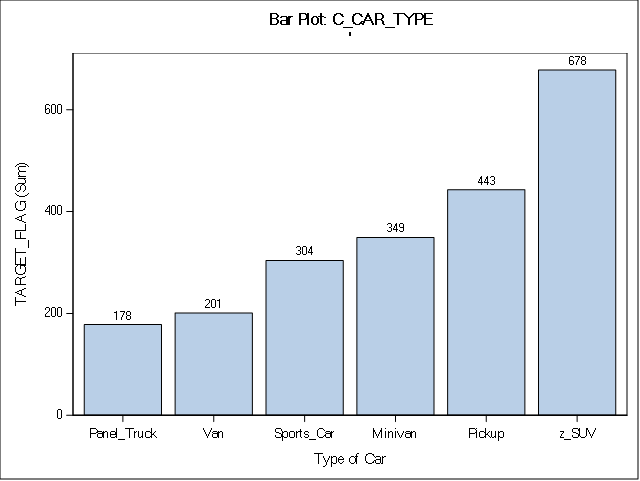
\includegraphics[height=3.95833in]{images/bar_cartype.png}

\paragraph{Figure 3.1.2 Bar Plot:
Education}\label{figure-3.1.2-bar-plot-education}

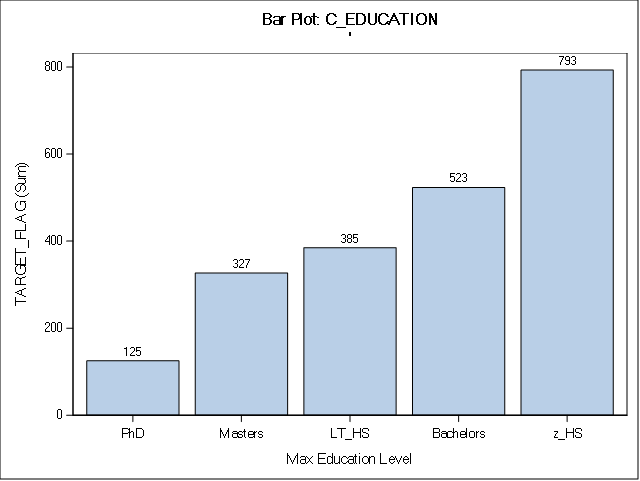
\includegraphics[height=3.95833in]{images/bar_education.png}

\newpage

\paragraph{Figure 3.1.3 Bar Plot: Job}\label{figure-3.1.3-bar-plot-job}

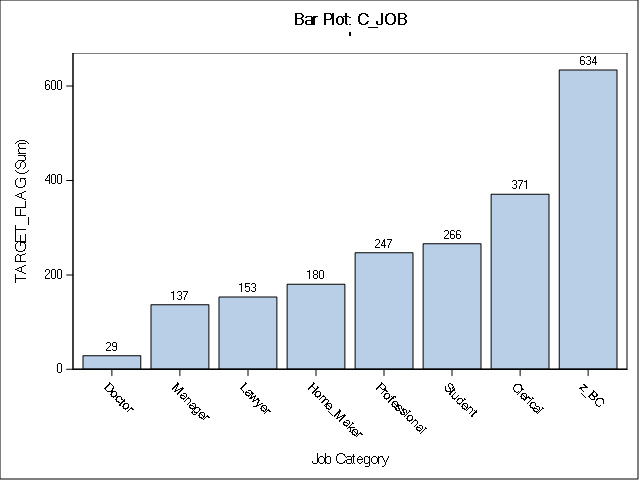
\includegraphics[height=3.95833in]{images/bar_job.png}

\paragraph{Figure 3.1.4 Bar Plot: Sex}\label{figure-3.1.4-bar-plot-sex}

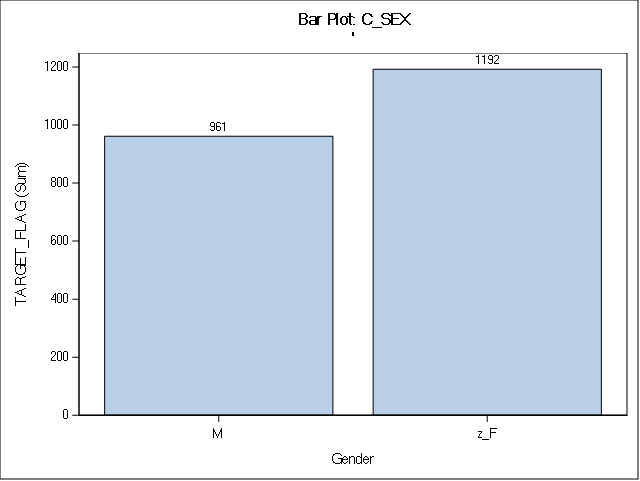
\includegraphics[height=3.95833in]{images/bar_sex.png}

\newpage

\paragraph{Figure 3.1.5 Histogram:
Age}\label{figure-3.1.5-histogram-age}

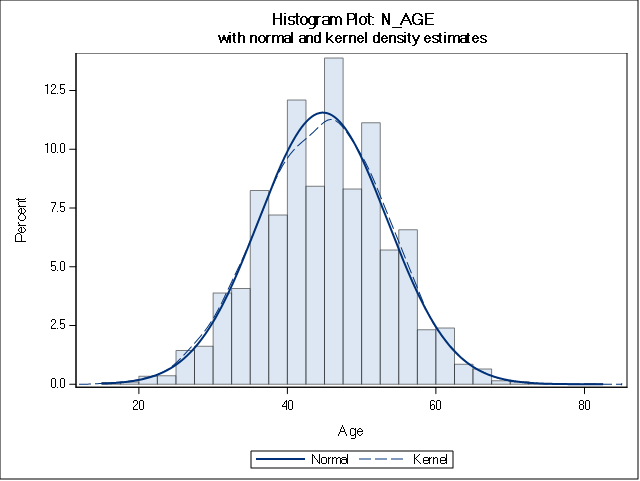
\includegraphics[height=3.95833in]{images/hist_age.png}

\paragraph{Figure 3.1.6 Box Plot: Age}\label{figure-3.1.6-box-plot-age}

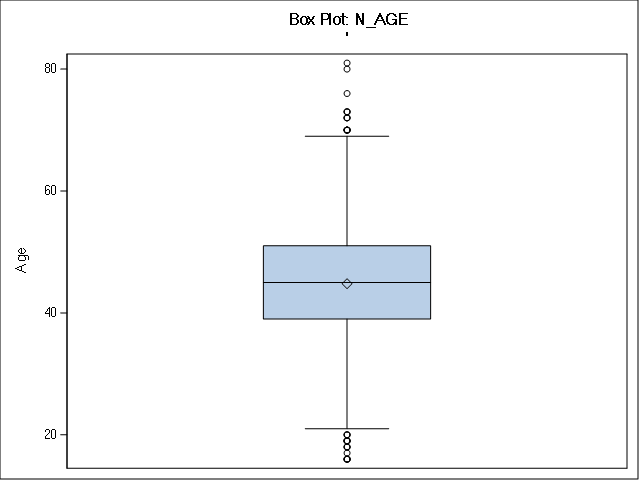
\includegraphics[height=3.95833in]{images/box_age.png}

\newpage

\paragraph{Figure 3.1.7 Histogram:
Income}\label{figure-3.1.7-histogram-income}

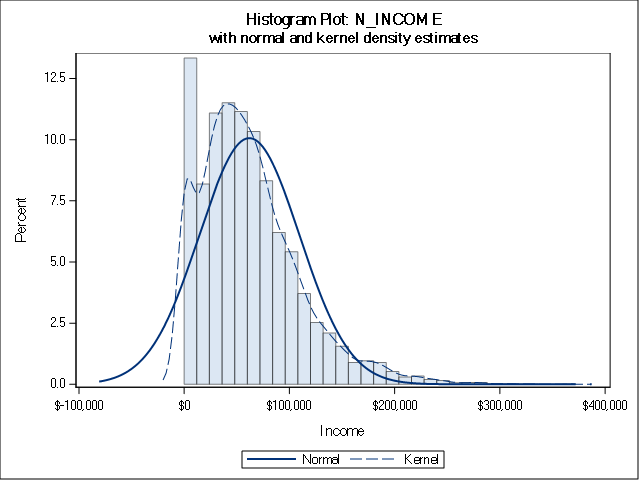
\includegraphics[height=3.95833in]{images/hist_income.png}

\paragraph{Figure 3.1.8 Box Plot:
Income}\label{figure-3.1.8-box-plot-income}

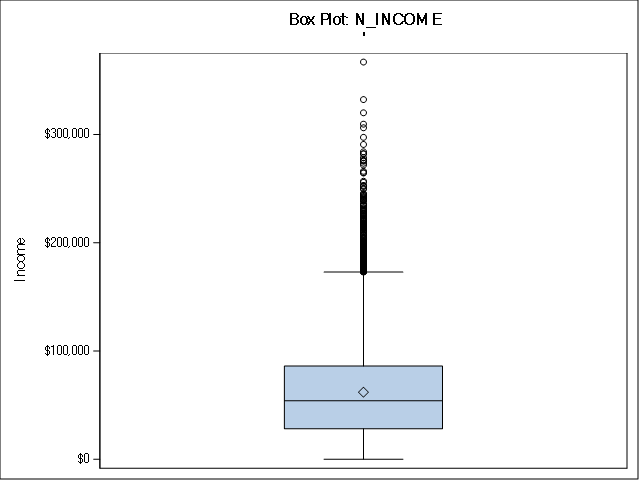
\includegraphics[height=3.95833in]{images/box_income.png}

\newpage

In terms of vehicle characteristics, we can see that the dataset has a
higher representation of those who drive a SUV or pickup vehicle
compared to those who drive a van or panel truck. In terms of driver
characteristics, we can see that the majority of drivers have a lower
level of education, tend to be unemployed or employed in
non-professional roles, and are generally female rather than male.

We note that few of the numeric variables exhibit a normal shaped
distribution. In-fact, N\_AGE was found to have the most normal shaped
distribution, while the remaining variables were found to have varying
degrees of skew. Our initial concerns of the presence of zero-inflated
data were also confirmed from the above exploratory analysis, with many
variables, including N\_INCOME, having a greater representation of zero
values.

\subsection{3.2 Bivariate Data Analysis}\label{bivariate-data-analysis}

Since we intend on building a prediction model for both the chance of a
car accident as well as the value of accident, we have an interest in
those variables which have explanatory power over these variables. As
such, we use the SAS procedure `corr' to see if any of the numeric
variables have a high Pearson correlation coefficient in relation to
accident value. We also generate frequency tables for each of the
character variables against the flag which indicates whether there was a
car accident.

The table below summarizes the correlation coefficients between accident
value and each numeric variable.

\paragraph{Table 3.2.1: Correlations for Accident Value vs.~Numeric
Data}\label{table-3.2.1-correlations-for-accident-value-vs.numeric-data}

\begin{longtable}[]{@{}ll@{}}
\toprule
Variable & Correlation\tabularnewline
\midrule
\endhead
N\_KIDSDRIV & 0.05539\tabularnewline
N\_AGE & -0.04173\tabularnewline
N\_HOMEKIDS & 0.06199\tabularnewline
N\_YOJ & -0.02209\tabularnewline
N\_INCOME & -0.05831\tabularnewline
N\_HOME\_VAL & -0.0856\tabularnewline
N\_TRAVTIME & 0.02777\tabularnewline
N\_BLUEBOOK & -0.0047\tabularnewline
N\_TIF & -0.04648\tabularnewline
N\_OLDCLAIM & 0.07095\tabularnewline
N\_CLM\_FREQ & 0.11642\tabularnewline
N\_MVR\_PTS & 0.13787\tabularnewline
N\_CAR\_AGE & -0.05882\tabularnewline
\bottomrule
\end{longtable}

None of the continuous variables are reported to have a particularly
strong positive or negative correlation coefficient with the response
variable, with the greatest absolute correlation being reported by
`N\_MVR\_PTS' and `N\_CLM\_FREQ' at 0.14 and 0.12 respectively.
Interestingly, we see a very weak correlation between N\_BLUEBOOK and
accident value.

The tables below summarize the percentage of observations which
coincided with an accident for each level of a number of chosen
character variables.

\paragraph{Table 3.2.2: Freq Table for Accident Flag
vs.~Education}\label{table-3.2.2-freq-table-for-accident-flag-vs.education}

\begin{longtable}[]{@{}llllll@{}}
\toprule
C\_EDUCATION & \textless{}HighSchool & z\_HighSchool & Bachelors &
Masters & PhD\tabularnewline
\midrule
\endhead
\% which had accidents & 32\% & 34\% & 23\% & 20\% & 17\%\tabularnewline
\bottomrule
\end{longtable}

We can see that a greater share of drivers with a low level of education
were involved in an accident, compared to drivers with a high level of
education.

\paragraph{Table 3.2.3: Freq Table for Accident Flag
vs.~Job}\label{table-3.2.3-freq-table-for-accident-flag-vs.job}

\begin{longtable}[]{@{}lllllllll@{}}
\toprule
C\_JOB & z\_BlueCollar & Clerical & Student & Professional & HomeMaker &
Lawyer & Manager & Doctor\tabularnewline
\midrule
\endhead
\% which had accidents & 33\% & 29\% & 37\% & 22\% & 28\% & 18\% & 14\%
& 12\%\tabularnewline
\bottomrule
\end{longtable}

Likewise, we see that a greater share of student drivers and drivers in
non-professional employment were involved in an accident.

\paragraph{Table 3.2.4: Freq Table for Accident Flag
vs.~Urbanicity}\label{table-3.2.4-freq-table-for-accident-flag-vs.urbanicity}

\begin{longtable}[]{@{}lll@{}}
\toprule
C\_URBANICITY & Highly Urban/ Urban & z\_Highly
Rural/Rural\tabularnewline
\midrule
\endhead
\% which had accidents & 31\% & 7\%\tabularnewline
\bottomrule
\end{longtable}

Perhaps not surprisingly, a greater proportion of accidents occurred in
urban areas compared to rural areas.

\paragraph{Table 3.2.5: Freq Table for Accident Flag
vs.~Revoked}\label{table-3.2.5-freq-table-for-accident-flag-vs.revoked}

\begin{longtable}[]{@{}lll@{}}
\toprule
C\_REVOKED & Yes & No\tabularnewline
\midrule
\endhead
\% which had accidents & 44\% & 24\%\tabularnewline
\bottomrule
\end{longtable}

And finally, we can see that those divers who had their licence revoked
within the past seven years had a much greater share of accidents.

\section{4 Data Preparation}\label{data-preparation}

The data preparation routine for this assessment follows a four step
process for numeric variables. This includes 1) identifying and
correcting any data errors, 2) trimming variables to account for
outliers, 3) imputing variables to account for missing values, and
finally, 4) performing a log transformation of all existing and newly
created variables. Note that during this process, new dummy variables
are created in order to reflect any identified outlier or missing
observations.

\subsection{4.1 Data Errors}\label{data-errors}

We note that the only data error found within this dataset is the -3
observation for N\_CAR\_AGE. Hence, we have replaced this observation
with its absolute value as a first step of the data preparation routine.
The N\_CAR\_AGE variable will include this replaced observation for all
subsequently derived variables.

\subsection{4.2 Data Outliers}\label{data-outliers}

From the univariate and bivariate analysis, we have identified that the
majority of numeric variables are in-fact zero-inflated and/or suffer
from outlier observations. A review of the percentiles for each variable
confirms this, with a rather large gap between the min, max and the 1st
and 99th percentile for each variable. A summary of percentiles for each
variable can be found in the table below.

\newpage

\paragraph{Table 4.1: Quantiles
Summary}\label{table-4.1-quantiles-summary}

\begin{longtable}[]{@{}llllllllllll@{}}
\toprule
& Min & 0.01 & 0.05 & 0.1 & 0.25 & 0.5 & 0.75 & 0.9 & 0.95 & 0.99 &
Max\tabularnewline
\midrule
\endhead
N\_KIDSDRIV & 0 & 0 & 0 & 0 & 0 & 0 & 0 & 1 & 1 & 2 & 4\tabularnewline
N\_AGE & 16 & 25 & 30 & 34 & 39 & 45 & 51 & 56 & 59 & 64 &
81\tabularnewline
N\_HOMEKIDS & 0 & 0 & 0 & 0 & 0 & 0 & 1 & 3 & 3 & 4 & 5\tabularnewline
N\_YOJ & 0 & 0 & 0 & 5 & 9 & 11 & 13 & 15 & 15 & 17 & 23\tabularnewline
N\_INCOME & 0 & 0 & 0 & 4362 & 28094 & 54028 & 86021 & 123217 & 152283 &
215536 & 367030\tabularnewline
N\_HOME\_VAL & 0 & 0 & 0 & 0 & 0 & 161160 & 238724 & 316587 & 374931 &
500309 & 885282\tabularnewline
N\_TRAVTIME & 5 & 5 & 7 & 13 & 22 & 33 & 44 & 54 & 60 & 75 &
142\tabularnewline
N\_BLUEBOOK & 1500 & 1500 & 4900 & 6000 & 9280 & 14440 & 20850 & 27460 &
31110 & 39090 & 69740\tabularnewline
N\_TIF & 1 & 1 & 1 & 1 & 1 & 4 & 7 & 11 & 13 & 17 & 25\tabularnewline
N\_OLDCLAIM & 0 & 0 & 0 & 0 & 0 & 0 & 4636 & 9583 & 27090 & 42820 &
57037\tabularnewline
N\_CLM\_FREQ & 0 & 0 & 0 & 0 & 0 & 0 & 2 & 3 & 3 & 4 & 5\tabularnewline
N\_MVR\_PTS & 0 & 0 & 0 & 0 & 0 & 1 & 3 & 5 & 6 & 8 & 13\tabularnewline
N\_CAR\_AGE & -3 & 1 & 1 & 1 & 1 & 8 & 12 & 16 & 18 & 21 &
28\tabularnewline
\bottomrule
\end{longtable}

For this assessment, we have elected to generate trimmed copies of each
numeric variable by their 1st/99th and 10th/90th percentiles. Trimmed
variables include the suffix '\_T99' and '\_T90' respectively. Based on
the quantile summary above, we note that the majority of variables which
are trimmed by their 1st/99th percentiles will retain zero value
observations, while the majority of variables which are trimmed by their
10th/90th percentiles will see an elimination of zero value
observations. A new set of dummy variables are also created in order to
capture those variables which were identified as having outlier
observations according to the percentile threshold discussed above.
These dummy variables include the suffix '\_OF'.

\subsection{4.3 Missing Data}\label{missing-data}

Following introducing copies of trimmed numeric variables, we then look
towards imputing values for missing observations. By recalculating
statistical measures for each variable after trimming, we are able to
avoid imputing skewed values for those variables which have been trimmed
into each variable. For this assessment, we generate new imputed
variables based on that variable's median value. Note that in order to
simplify the SAS logic used for this assessment, all variables will
include the suffix '\_IME', however only those variables shown to have
missing observations in the previous sections have actually received
imputation. A new set of dummy variables are also created in order to
capture those variables which were identified as having missing
observations. These variables include the suffix '\_MF'.

\subsection{4.4 Data Transformation}\label{data-transformation}

We perform a natural logarithm transformation of each of the numeric
variables. Variables which have been transformed include the suffix
'\_LN'. Such a transformation will help penalize extreme values and may
provide an improved fit within subsequent regression models. This
transformation is performed for all of the newly created non-dummy
variables discussed above.

\subsection{4.5 Dummy Variables}\label{dummy-variables}

Finally, we create a number of dummy variables based on bins of numeric
variables and add these to the prepared numeric variables discussed
above. The dummy variables created for this assessment are detailed in
the table below.

\newpage

\paragraph{Table 4.2: Dummy Variable
Summary}\label{table-4.2-dummy-variable-summary}

\begin{longtable}[]{@{}ll@{}}
\toprule
Variable & Criteria\tabularnewline
\midrule
\endhead
N\_AGE\_Risk\_Yes & (N\_AGE \textless{}= 30\tabularnewline
N\_AGE\_Risk\_No & (N\_AGE\_Risk\_Yes = 0)\tabularnewline
N\_BLUEBOOK\_Hi & (N\_BLUEBOOK \textgreater{}= 27000)\tabularnewline
N\_BLUEBOOK\_Lo & (N\_BLUEBOOK\_Hi = 0)\tabularnewline
N\_CLM\_FREQ\_No & (N\_CLM\_FREQ = 0)\tabularnewline
N\_CLM\_FREQ\_Yes & (N\_CLM\_FREQ \textgreater{} 0)\tabularnewline
N\_CLM\_FREQ\_Hi & (N\_CLM\_FREQ \textgreater{}= 2)\tabularnewline
N\_CLM\_FREQ\_Lo & (N\_CLM\_FREQ\_Hi = 0)\tabularnewline
N\_HOMEKIDS\_No & (N\_HOMEKIDS = 0)\tabularnewline
N\_HOMEKIDS\_Yes & (N\_HOMEKIDS \textgreater{} 0)\tabularnewline
N\_INCOME\_No & (N\_INCOME = 0)\tabularnewline
N\_INCOME\_Yes & (N\_INCOME \textgreater{} 0)\tabularnewline
N\_INCOME\_Hi & (N\_INCOME \textgreater{}= 85000)\tabularnewline
N\_INCOME\_Lo & (N\_INCOME\_Hi = 0)\tabularnewline
N\_KIDSDRIV\_No & (N\_KIDSDRIV = 0)\tabularnewline
N\_KIDSDRIV\_Yes & (N\_KIDSDRIV \textgreater{} 0)\tabularnewline
N\_MVR\_PTS\_No & (N\_MVR\_PTS = 0)\tabularnewline
N\_MVR\_PTS\_Yes & (N\_MVR\_PTS \textgreater{} 0)\tabularnewline
N\_MVR\_PTS\_Hi & (N\_MVR\_PTS \textgreater{}= 4)\tabularnewline
N\_MVR\_PTS\_Lo & (N\_MVR\_PTS\_Hi = 0)\tabularnewline
N\_OLDCLAIM\_No & (N\_OLDCLAIM = 0)\tabularnewline
N\_OLDCLAIM\_Yes & (N\_OLDCLAIM \textgreater{} 0)\tabularnewline
N\_OLDCLAIM\_Hi & (N\_OLDCLAIM \textgreater{}= 9500)\tabularnewline
N\_OLDCLAIM\_Lo & (N\_OLDCLAIM\_Hi = 0)\tabularnewline
N\_RENTER\_Yes & (N\_HOME\_VAL \textless{}= 14400)\tabularnewline
N\_RENTER\_No & (N\_RENTER\_Yes = 0)\tabularnewline
N\_TRAVTIME\_Hi & (N\_TRAVTIME \textgreater{}= 50)\tabularnewline
N\_TRAVTIME\_Lo & (N\_TRAVTIME\_Hi = 0)\tabularnewline
\bottomrule
\end{longtable}

Note that the newly created dummy variables include an appropriate
suffix to reflect its criteria.

\section{5 Model Development}\label{model-development}

For this section, we build two different classes of regression model.
First, we build a linear regression model in order to predict the value
of an accident. Second, we build three logistic regression models in
order to predict the probability of a car accident.

\subsection{5.1 Model 0: Linear Regression (Stepwise Selection
Model)}\label{model-0-linear-regression-stepwise-selection-model}

From a pool of 13 numeric variables, only N\_BLUEBOOK and N\_CAR\_AGE
would seem to have reasonable justification for predicting accident
value, with the remaining 11 variables either having a greater
jusitification for predicting the probability of an accident or having
little justification for predicting either the value or probability of
an accident. As such, this assessment initially attempted to build a
linear regression model using only these two variables. However the fit
was found to be unsatisfactory both in terms of its goodness-of-fit and
due to failure of a number of OLS assumptions. As an alternative, this
assessment has elected to use an automated variable technique based on
stepwise selection to specify the linear regression model
(Model\_LinR\_S).

For the linear regression model with stepwise selection
(Model\_LinR\_S), we elected to use a SLENTRY value of 0.10. This
indicates that variables should only be added to the specification if
they have a significance level (p-value) of less than 10\%. We also
elected to use a SLSTAY value of 0.10, which indicates that variables
should not be removed from the specification if they have a significance
level (p-value) less than 10\%.

Parameter estimates for the Model\_LinR\_S are shown below.

\paragraph{Table 5.1.1: Linear Regression (Stepwise Selection Model)
Parameter
Estimates}\label{table-5.1.1-linear-regression-stepwise-selection-model-parameter-estimates}

\begin{longtable}[]{@{}lllllll@{}}
\toprule
Variable & DF & Est. & S.E. & t Value & \$\text{Pr} \textgreater{} &
t\tabularnewline
\midrule
\endhead
Intercept & 1 & 607.45408 & 407.17719 & 1.49 & 0.1358 & 0\tabularnewline
N\_MVR\_PTS\_OF & 1 & 1033.99599 & 587.13791 & 1.76 & 0.0783 &
1.1402\tabularnewline
N\_AGE\_Risk\_Yes & 1 & 515.35611 & 180.30355 & 2.86 & 0.0043 &
1.05295\tabularnewline
N\_CLM\_FREQ\_No & 1 & -759.93781 & 119.31081 & -6.37 & \textless{}.0001
& 1.29417\tabularnewline
N\_HOMEKIDS\_Yes & 1 & 287.91233 & 126.02274 & 2.28 & 0.0224 &
1.38916\tabularnewline
N\_INCOME\_Lo & 1 & 363.19203 & 132.53969 & 2.74 & 0.0062 &
1.23457\tabularnewline
N\_KIDSDRIV\_Yes & 1 & 569.54126 & 181.63075 & 3.14 & 0.0017 &
1.33804\tabularnewline
N\_RENTER\_Yes & 1 & 548.74609 & 108.68295 & 5.05 & \textless{}.0001 &
1.01356\tabularnewline
N\_BLUEBOOK\_IME & 1 & 0.01586 & 0.00645 & 2.46 & 0.0139 &
1.12956\tabularnewline
N\_CAR\_AGE\_T90\_IME & 1 & -33.37866 & 9.94921 & -3.35 & 0.0008 &
1.1553\tabularnewline
N\_MVR\_PTS\_IME & 1 & 175.36712 & 28.57688 & 6.14 & \textless{}.0001 &
1.44367\tabularnewline
N\_TIF\_IME\_LN & 1 & -271.31906 & 72.49254 & -3.74 & 0.0002 &
1.00219\tabularnewline
N\_TRAVTIME\_T99\_IME\_LN & 1 & 248.96682 & 90.88666 & 2.74 & 0.0062 &
1.0027\tabularnewline
\bottomrule
\end{longtable}

For Model\_LinR\_S, the majority of coefficient estimates have
significant p-values at the 95\% level, allowing us to reject the null
hypothesis and conclude that each have non-zero coefficients. The only
exception is the coefficient estimate for the outlier flag
N\_MVR\_PTS\_OF. However, it is difficult to assess the polarity of
coefficient estimates, as many of the included variables have little
justification for predicting the value of a car accident.

Goodness-of-fit information for Model\_LinR\_S is shown below.

\paragraph{Table 5.1.2: Linear Regression Stepwise Selection Model)
Analysis of
Variance}\label{table-5.1.2-linear-regression-stepwise-selection-model-analysis-of-variance}

\begin{longtable}[]{@{}llllll@{}}
\toprule
Source & DF & Sum of Squares & Mean Square & F Value & Pr \textgreater{}
F\tabularnewline
\midrule
\endhead
Model & 12 & 7178263642 & 598188637 & 28.11 &
\textless{}.0001\tabularnewline
Error & 8148 & 1.73385E+11 & 21279474 & &\tabularnewline
Corrected Total & 8160 & 1.80563E+11 & & &\tabularnewline
\bottomrule
\end{longtable}

The model has reported a large F-value suggesting that the observations
and regression differ from the grand mean. Likewise, the F-value has a
highly significant p-value under the null hypothesis that there is no
linear relationship between the predictor and response variable.

Model performance statistics for Model\_LinR\_S are shown below.

\paragraph{Table 5.1.3: Linear Regression (Stepwise Selection Model)
Performance
Metrics}\label{table-5.1.3-linear-regression-stepwise-selection-model-performance-metrics}

\begin{longtable}[]{@{}llll@{}}
\toprule
Measure & Statistic & Measure & Statistic\tabularnewline
\midrule
\endhead
MSE & 21279474 & R-Square & 0.0398\tabularnewline
MAE & 2033.08 & Adj R-Sq & 0.0383\tabularnewline
Root MSE & 4612.96797 & C(p) & 13\tabularnewline
Dependent Mean & 1504.32465 & AIC & 137715.611\tabularnewline
Coeff Var & 306.6471 & BIC & 137717.653\tabularnewline
\bottomrule
\end{longtable}

The R-square value above suggests that Model\_LinR\_S explains only
\textasciitilde{}4\% of the variability in TARGET\_AMT using each of the
included predictor variables. The adjusted R-squared value also
indicates a similar level of explanatory power.

\subsection{5.2 Model 1: Logistic Regression (Subjective
Model)}\label{model-1-logistic-regression-subjective-model}

For the first logistic regression model (Model\_LogR\_Subj), we include
only those variables which have a reasonable justification for
predicting the probability of a car accident. We build on this by
including missing variable flags for retained variables which were shown
to have missing variables and include outlier flags for retained
variables which were shown to have a large amount of outliers. Finally,
we removed any variables from this specification which were found to be
highly insignificant.

Parameter estimates for the Model\_LogR\_Subj are shown below.

\paragraph{Table 5.2.1: Logistic Regression (Subjective Model) Parameter
Estimates}\label{table-5.2.1-logistic-regression-subjective-model-parameter-estimates}

\begin{longtable}[]{@{}lllllll@{}}
\toprule
Parameter & & DF & Est. & S.E. & Wald ChiSq & Pr \textgreater{}
ChiSq\tabularnewline
\midrule
\endhead
Intercept & & 1 & -1.5376 & 0.2464 & 38.9366 &
\textless{}.0001\tabularnewline
C\_CAR\_USE & Commercial & 1 & 0.7095 & 0.0779 & 82.9619 &
\textless{}.0001\tabularnewline
C\_EDUCATION & Bachelors & 1 & -0.4024 & 0.0832 & 23.4094 &
\textless{}.0001\tabularnewline
C\_EDUCATION & LT\_HS & 1 & -0.0356 & 0.092 & 0.1497 &
0.6988\tabularnewline
C\_EDUCATION & Masters & 1 & -0.3458 & 0.1465 & 5.5672 &
0.0183\tabularnewline
C\_EDUCATION & PhD & 1 & -0.0547 & 0.2025 & 0.0729 &
0.7871\tabularnewline
C\_JOB & Clerical & 1 & 0.0825 & 0.1034 & 0.6366 & 0.425\tabularnewline
C\_JOB & Doctor & 1 & -0.8406 & 0.2974 & 7.9879 & 0.0047\tabularnewline
C\_JOB & Home\_Maker & 1 & 0.0623 & 0.1441 & 0.1871 &
0.6653\tabularnewline
C\_JOB & Lawyer & 1 & -0.1798 & 0.185 & 0.9449 & 0.331\tabularnewline
C\_JOB & Manager & 1 & -0.8386 & 0.1343 & 39.014 &
\textless{}.0001\tabularnewline
C\_JOB & Professional & 1 & -0.1728 & 0.1139 & 2.3034 &
0.1291\tabularnewline
C\_JOB & Student & 1 & 0.0464 & 0.1216 & 0.1454 & 0.7029\tabularnewline
C\_MSTATUS & Yes & 1 & -0.7483 & 0.0611 & 149.7778 &
\textless{}.0001\tabularnewline
C\_REVOKED & No & 1 & -0.9076 & 0.0934 & 94.462 &
\textless{}.0001\tabularnewline
C\_URBANICITY & Urban & 1 & 2.2928 & 0.1116 & 422.4525 &
\textless{}.0001\tabularnewline
N\_AGE\_IME & & 1 & -0.00958 & 0.00359 & 7.1237 & 0.0076\tabularnewline
N\_CLM\_FREQ\_IME & & 1 & 0.2169 & 0.0294 & 54.5098 &
\textless{}.0001\tabularnewline
N\_INCOME\_IME & & 1 & -0.00000794 & 0.00000118 & 45.2549 &
\textless{}.0001\tabularnewline
N\_KIDSDRIV\_IME & & 1 & 0.4864 & 0.0631 & 59.4666 &
\textless{}.0001\tabularnewline
N\_MVR\_PTS\_IME & & 1 & 0.1123 & 0.0149 & 56.7098 &
\textless{}.0001\tabularnewline
N\_OLDCLAIM\_IME & & 1 & -0.00002 & 0.000004046 & 14.4407 &
0.0001\tabularnewline
N\_TIF\_IME & & 1 & -0.0531 & 0.00754 & 49.6228 &
\textless{}.0001\tabularnewline
N\_TRAVTIME\_IME & & 1 & 0.0142 & 0.00192 & 54.7967 &
\textless{}.0001\tabularnewline
N\_AGE\_MF & & 1 & 2.4375 & 1.1897 & 4.1974 & 0.0405\tabularnewline
N\_INCOME\_MF & & 1 & -1.1339 & 0.5248 & 4.6686 & 0.0307\tabularnewline
N\_INCOME\_OF & & 1 & 1.1128 & 0.5118 & 4.7269 & 0.0297\tabularnewline
N\_KIDSDRIV\_OF & & 1 & -0.5083 & 0.347 & 2.1456 & 0.143\tabularnewline
N\_MVR\_PTS\_OF & & 1 & 0.5927 & 0.3271 & 3.2841 & 0.07\tabularnewline
\bottomrule
\end{longtable}

We interpret coefficients as the variables' influence on the likelihood
of a crash. That is, an increase in the value of any variable with a
positive coefficient is estimated to result in an increase in likelihood
of a crash. With this in mind, we are critical of a number of
coefficient estimates for the subjective model. For instance, we would
not expect an increase in the payout of previous claims
(N\_OLDCLAIM\_IME) to result in a decrease in likelihood of a crash.

Goodness-of-fit information for Model\_LogR\_Subj is shown below.

\paragraph{Table 5.2.2: Logistic Regression (Subjective Model) Test of
Global Null
Hypothesis}\label{table-5.2.2-logistic-regression-subjective-model-test-of-global-null-hypothesis}

\begin{longtable}[]{@{}llll@{}}
\toprule
Test & Chi-Square & DF & Pr \textgreater{} ChiSq\tabularnewline
\midrule
\endhead
Likelihood Ratio & 1870.7673 & 28 & \textless{}.0001\tabularnewline
Score & 1673.6328 & 28 & \textless{}.0001\tabularnewline
Wald & 1271.9264 & 28 & \textless{}.0001\tabularnewline
\bottomrule
\end{longtable}

We compute the Kolmogorov-Smirnov (KS) statistic for the model by
performing a random sampling for test and validation using the SAS
NPAR1WAY procedure. The results, along with model performance criteria
are shown below.

\paragraph{Table 5.2.3: Logistic Regression (Subjective Model)
Performance
Metrics}\label{table-5.2.3-logistic-regression-subjective-model-performance-metrics}

\begin{longtable}[]{@{}lll@{}}
\toprule
Criterion & Intercept Only & Intercept and Covariates\tabularnewline
\midrule
\endhead
AIC & 8818.622 & 7003.854\tabularnewline
SC & 8825.562 & 7205.129\tabularnewline
-2 Log L & 8816.622 & 6945.854\tabularnewline
\bottomrule
\end{longtable}

\begin{longtable}[]{@{}llll@{}}
\toprule
Measure & Statistic & Measure & Statistic\tabularnewline
\midrule
\endhead
KS & 0.203568 & D & 0.461715\tabularnewline
KSa & 17.787425 & Pr \textgreater{} KSa &
\textless{}.0001\tabularnewline
\bottomrule
\end{longtable}

These statistics will be helpful in drawing a comparison between
alternative model estimations.

Finally, we can observe the ROC curve for this model.

\paragraph{Figure 5.2.1 ROC Curve (Subjective
Model)}\label{figure-5.2.1-roc-curve-subjective-model}

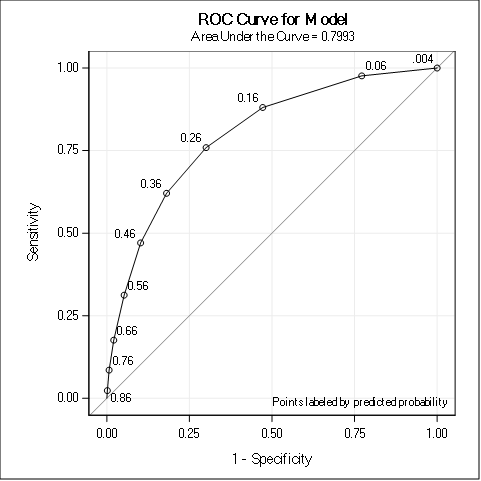
\includegraphics[height=3.54167in]{images/roc_subj.png}

The ROC curve suggests that Model\_LogR\_Subj has 0.7993 coverage and
lies significantly above the diagonal.

\subsection{5.3 Model 2: Logistic Regression (Forward Selection
Model)}\label{model-2-logistic-regression-forward-selection-model}

We leverage automated variables selection techniques to specify the
remaining two logistic regression models. For the first, we use the
forward selection technique for variable selection (Model\_LogR\_F).
Note that we elected to use a SLENTRY value of 0.15 as part of this
technique, which indicates that variables should only be added to the
specification if their coefficient estimation has a significance level
(p-value) less than 15\%.

Parameter estimates for Model\_LogR\_F are shown below.

\paragraph{Table 5.3.1: Logistic Regression (Forward Selection Model)
Parameter
Estimates}\label{table-5.3.1-logistic-regression-forward-selection-model-parameter-estimates}

\begin{longtable}[]{@{}lllllll@{}}
\toprule
Parameter & & DF & Est. & S.E. & Wald ChiSq & Pr \textgreater{}
ChiSq\tabularnewline
\midrule
\endhead
Intercept & & 1 & 2.2393 & 0.6232 & 12.9132 & 0.0003\tabularnewline
C\_PARENT1 & No & 1 & -0.1633 & 0.1265 & 1.6672 & 0.1966\tabularnewline
C\_MSTATUS & Yes & 1 & -0.5654 & 0.0942 & 36.0183 &
\textless{}.0001\tabularnewline
C\_EDUCATION & Bachelors & 1 & -0.3997 & 0.0851 & 22.0644 &
\textless{}.0001\tabularnewline
C\_EDUCATION & LT\_HS & 1 & -0.00154 & 0.0963 & 0.0003 &
0.9872\tabularnewline
C\_EDUCATION & Masters & 1 & -0.3613 & 0.1504 & 5.7738 &
0.0163\tabularnewline
C\_EDUCATION & PhD & 1 & -0.1091 & 0.2029 & 0.2892 &
0.5907\tabularnewline
C\_JOB & Clerical & 1 & 0.0894 & 0.1081 & 0.684 & 0.4082\tabularnewline
C\_JOB & Doctor & 1 & -0.944 & 0.3028 & 9.7165 & 0.0018\tabularnewline
C\_JOB & Home\_Maker & 1 & -0.3276 & 0.1679 & 3.8083 &
0.051\tabularnewline
C\_JOB & Lawyer & 1 & -0.1902 & 0.1919 & 0.9825 & 0.3216\tabularnewline
C\_JOB & Manager & 1 & -0.9099 & 0.1419 & 41.103 &
\textless{}.0001\tabularnewline
C\_JOB & Professional & 1 & -0.1775 & 0.1218 & 2.1233 &
0.1451\tabularnewline
C\_JOB & Student & 1 & -0.4303 & 0.1483 & 8.4246 & 0.0037\tabularnewline
C\_CAR\_USE & Commercial & 1 & 0.7771 & 0.0949 & 67.0621 &
\textless{}.0001\tabularnewline
C\_CAR\_TYPE & Minivan & 1 & -0.7607 & 0.0882 & 74.3163 &
\textless{}.0001\tabularnewline
C\_CAR\_TYPE & Panel\_Truck & 1 & -0.12 & 0.174 & 0.4755 &
0.4905\tabularnewline
C\_CAR\_TYPE & Pickup & 1 & -0.0981 & 0.0967 & 1.0278 &
0.3107\tabularnewline
C\_CAR\_TYPE & Sports\_Car & 1 & 0.1848 & 0.1005 & 3.3811 &
0.0659\tabularnewline
C\_CAR\_TYPE & Van & 1 & -0.1662 & 0.1304 & 1.6258 &
0.2023\tabularnewline
C\_REVOKED & No & 1 & -0.9284 & 0.0974 & 90.8318 &
\textless{}.0001\tabularnewline
C\_URBANICITY & Urban & 1 & 2.3624 & 0.1141 & 428.3742 &
\textless{}.0001\tabularnewline
N\_AGE\_MF & & 1 & 1.6736 & 1.2018 & 1.9392 & 0.1638\tabularnewline
N\_CAR\_AGE\_MF & & 1 & 0.2066 & 0.1237 & 2.7884 & 0.0949\tabularnewline
N\_AGE\_Risk\_Yes & & 1 & 0.5679 & 0.1005 & 31.91 &
\textless{}.0001\tabularnewline
N\_BLUEBOOK\_Hi & & 1 & -0.5269 & 0.1636 & 10.3686 &
0.0013\tabularnewline
N\_CLM\_FREQ\_Yes & & 1 & 0.6429 & 0.0823 & 61.0209 &
\textless{}.0001\tabularnewline
N\_HOMEKIDS\_No & & 1 & -0.3472 & 0.1399 & 6.1614 &
0.0131\tabularnewline
N\_INCOME\_Hi & & 1 & -0.3739 & 0.1067 & 12.2746 & 0.0005\tabularnewline
N\_MVR\_PTS\_Hi & & 1 & -0.4519 & 0.1327 & 11.5988 &
0.0007\tabularnewline
N\_BLUEBOOK\_T90\_IME & & 1 & 0.000017 & 0.000007 & 5.0557 &
0.0245\tabularnewline
N\_HOMEKIDS\_T99\_IME & & 1 & -0.1043 & 0.0551 & 3.5836 &
0.0584\tabularnewline
N\_HOME\_VAL\_T99\_IME & & 1 & -0.0000003 & 7.108E-07 & 0.2316 &
0.6304\tabularnewline
N\_MVR\_PTS\_IME & & 1 & 0.1617 & 0.0256 & 39.8646 &
\textless{}.0001\tabularnewline
N\_OLDCLAIM\_IME & & 1 & -0.00002 & 0.0000044 & 22.6314 &
\textless{}.0001\tabularnewline
N\_TRAVTIME\_T99\_IME & & 1 & 0.0169 & 0.00208 & 65.6788 &
\textless{}.0001\tabularnewline
N\_YOJ\_T99\_IME & & 1 & 0.0174 & 0.0113 & 2.4011 &
0.1213\tabularnewline
N\_BLUEBOOK\_T99\_IME\_L & & 1 & -0.3568 & 0.0656 & 29.6028 &
\textless{}.0001\tabularnewline
N\_HOME\_VAL\_T99\_IME\_L & & 1 & -0.0238 & 0.0137 & 3.0299 &
0.0817\tabularnewline
N\_INCOME\_T99\_IME\_LN & & 1 & -0.08 & 0.0183 & 19.0906 &
\textless{}.0001\tabularnewline
N\_KIDSDRIV\_IME\_LN & & 1 & 0.7506 & 0.1129 & 44.2155 &
\textless{}.0001\tabularnewline
N\_TIF\_IME\_LN & & 1 & -0.3262 & 0.0436 & 56.0911 &
\textless{}.0001\tabularnewline
\bottomrule
\end{longtable}

We can see that the high SLENTRY value has resulted in including a
number of insignificant variables within the specification. We are again
cautious in the interpretation of a number of variables noting their
unexpected polarity.

Goodness-of-fit information for Model\_LogR\_F is shown below.

\paragraph{Table 5.3.2: Logistic Regression (Forward Selection Model)
Test of Global Null
Hypothesis}\label{table-5.3.2-logistic-regression-forward-selection-model-test-of-global-null-hypothesis}

\begin{longtable}[]{@{}llll@{}}
\toprule
Test & Chi-Square & DF & Pr \textgreater{} ChiSq\tabularnewline
\midrule
\endhead
Likelihood Ratio & 2177.8624 & 41 & \textless{}.0001\tabularnewline
Score & 1904.0449 & 41 & \textless{}.0001\tabularnewline
Wald & 1388.3069 & 41 & \textless{}.0001\tabularnewline
\bottomrule
\end{longtable}

As with the previous model, we show performance statistics for
Model\_LogR\_F below. We can see an improvement in both the AIC and KS
statistics for this model, even though it has a much higher variable
count.

\paragraph{Table 5.3.3: Logistic Regression (Forward Selection Model)
Performance
Metrics}\label{table-5.3.3-logistic-regression-forward-selection-model-performance-metrics}

\begin{longtable}[]{@{}lll@{}}
\toprule
Criterion & Intercept Only & Intercept and Covariates\tabularnewline
\midrule
\endhead
AIC & 8818.622 & 6722.759\tabularnewline
SC & 8825.562 & 7014.26\tabularnewline
-2 Log L & 8816.622 & 6638.759\tabularnewline
\bottomrule
\end{longtable}

\begin{longtable}[]{@{}llll@{}}
\toprule
Measure & Statistic & Measure & Statistic\tabularnewline
\midrule
\endhead
KS & 0.219433 & D & 0.497699\tabularnewline
KSa & 19.173695 & Pr \textgreater{} KSa &
\textless{}.0001\tabularnewline
\bottomrule
\end{longtable}

Finally, we can observe the ROC curve for this model.

\newpage

\paragraph{Figure 5.3.1 ROC Curve (Forward Selection
Model)}\label{figure-5.3.1-roc-curve-forward-selection-model}

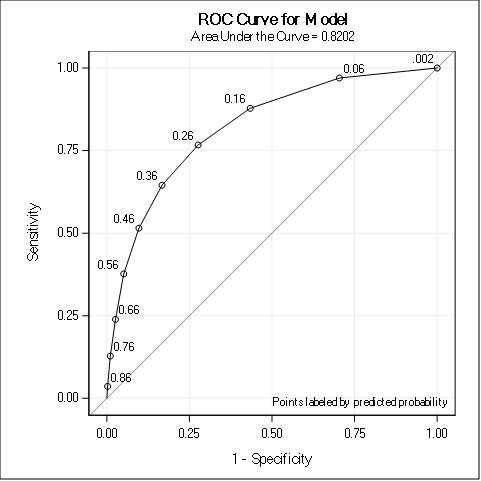
\includegraphics[height=3.54167in]{images/roc_f.png}

The ROC curve suggests that Model\_LogR\_F has 0.8202 coverage and lies
significantly above the diagonal. This is an improvement over the ROC
curve for Model\_LogR\_Subj.

\subsection{5.4 Model 3: Logistic Regression (Stepwise Selection
Model)}\label{model-3-logistic-regression-stepwise-selection-model}

For the final logistic regression model, we again use the stepwise
technique for variable selection (Model\_LogR\_S). Note that we elected
to use a SLENTRY value of 0.02 as part of this technique, which
indicates that variables should only be added to the specification if
they have a significance level (p-value) of less than 2\%. We also
elected to use a SLSTAY value of 0.02, which indicates that variables
should not be removed from the specification if they have a significance
level (p-value) less than 2\%.

Parameter estimates for Model\_LogR\_S are shown below.

\paragraph{Table 5.4.1: Logistic Regression (Stepwise Selection Model)
Parameter
Estimates}\label{table-5.4.1-logistic-regression-stepwise-selection-model-parameter-estimates}

\begin{longtable}[]{@{}lllllll@{}}
\toprule
Parameter & & DF & Est. & S.E. & Wald ChiSq & Pr \textgreater{}
ChiSq\tabularnewline
\midrule
\endhead
Intercept & & 1 & 2.0478 & 0.6079 & 11.3476 & 0.0008\tabularnewline
C\_PARENT1 & No & 1 & -0.3078 & 0.1 & 9.4681 & 0.0021\tabularnewline
C\_MSTATUS & Yes & 1 & -0.5291 & 0.0839 & 39.7965 &
\textless{}.0001\tabularnewline
C\_EDUCATION & Bachelors & 1 & -0.3933 & 0.0847 & 21.5486 &
\textless{}.0001\tabularnewline
C\_EDUCATION & LT\_HS & 1 & -0.013 & 0.0958 & 0.0183 &
0.8923\tabularnewline
C\_EDUCATION & Masters & 1 & -0.3638 & 0.1499 & 5.8884 &
0.0152\tabularnewline
C\_EDUCATION & PhD & 1 & -0.1052 & 0.2028 & 0.2693 &
0.6038\tabularnewline
C\_JOB & Clerical & 1 & 0.0749 & 0.1071 & 0.4899 & 0.484\tabularnewline
C\_JOB & Doctor & 1 & -0.9423 & 0.3028 & 9.6875 & 0.0019\tabularnewline
C\_JOB & Home\_Maker & 1 & -0.3622 & 0.1652 & 4.8072 &
0.0283\tabularnewline
C\_JOB & Lawyer & 1 & -0.1861 & 0.1915 & 0.9436 & 0.3313\tabularnewline
C\_JOB & Manager & 1 & -0.912 & 0.1415 & 41.5138 &
\textless{}.0001\tabularnewline
C\_JOB & Professional & 1 & -0.1776 & 0.1215 & 2.1372 &
0.1438\tabularnewline
C\_JOB & Student & 1 & -0.3516 & 0.1441 & 5.9505 & 0.0147\tabularnewline
C\_CAR\_USE & Commercial & 1 & 0.7603 & 0.0945 & 64.7697 &
\textless{}.0001\tabularnewline
C\_CAR\_TYPE & Minivan & 1 & -0.764 & 0.0881 & 75.2865 &
\textless{}.0001\tabularnewline
C\_CAR\_TYPE & Panel\_Truck & 1 & -0.1189 & 0.1735 & 0.4699 &
0.493\tabularnewline
C\_CAR\_TYPE & Pickup & 1 & -0.1055 & 0.0964 & 1.1959 &
0.2741\tabularnewline
C\_CAR\_TYPE & Sports\_Car & 1 & 0.1737 & 0.1003 & 3.0001 &
0.0833\tabularnewline
C\_CAR\_TYPE & Van & 1 & -0.1629 & 0.1299 & 1.5726 &
0.2098\tabularnewline
C\_REVOKED & No & 1 & -0.9242 & 0.0972 & 90.3173 &
\textless{}.0001\tabularnewline
C\_URBANICITY & Urban & 1 & 2.3598 & 0.114 & 428.3237 &
\textless{}.0001\tabularnewline
N\_AGE\_Risk\_Yes & & 1 & 0.6004 & 0.0994 & 36.4633 &
\textless{}.0001\tabularnewline
N\_BLUEBOOK\_Hi & & 1 & -0.5338 & 0.1636 & 10.6516 &
0.0011\tabularnewline
N\_CLM\_FREQ\_Yes & & 1 & 0.6365 & 0.0822 & 60.0212 &
\textless{}.0001\tabularnewline
N\_INCOME\_Hi & & 1 & -0.3263 & 0.1001 & 10.6235 & 0.0011\tabularnewline
N\_MVR\_PTS\_Hi & & 1 & -0.4492 & 0.1324 & 11.5101 &
0.0007\tabularnewline
N\_BLUEBOOK\_T90\_IME & & 1 & 0.000018 & 0.0000075 & 5.7881 &
0.0161\tabularnewline
N\_HOME\_VAL\_T99\_IME & & 1 & -0.000001 & 3.784E-07 & 14.0791 &
0.0002\tabularnewline
N\_MVR\_PTS\_IME & & 1 & 0.162 & 0.0255 & 40.2604 &
\textless{}.0001\tabularnewline
N\_OLDCLAIM\_IME & & 1 & -0.00002 & 0.0000044 & 21.8101 &
\textless{}.0001\tabularnewline
N\_TRAVTIME\_T99\_IME & & 1 & 0.0168 & 0.00208 & 65.1491 &
\textless{}.0001\tabularnewline
N\_BLUEBOOK\_T99\_IME\_L & & 1 & -0.3661 & 0.0652 & 31.5458 &
\textless{}.0001\tabularnewline
N\_INCOME\_T99\_IME\_LN & & 1 & -0.0597 & 0.0143 & 17.4061 &
\textless{}.0001\tabularnewline
N\_KIDSDRIV\_IME\_LN & & 1 & 0.7976 & 0.1023 & 60.7396 &
\textless{}.0001\tabularnewline
N\_TIF\_IME\_LN & & 1 & -0.3233 & 0.0435 & 55.3218 &
\textless{}.0001\tabularnewline
\bottomrule
\end{longtable}

Unlike the previous forward selection technique, the stepwise selection
technique has resulted in the inclusion of less insignificant variables.
Also unlike the manually specified model, the automated variable
selection techniques clearly have a greater preference for inclusion of
dummy variables created as part of the data preparation routine.

Goodness-of-fit information for Model\_LogR\_S is shown below.

\paragraph{Table 5.4.2: Logistic Regression (Stepwise Selection Model)
Test of Global Null
Hypothesis}\label{table-5.4.2-logistic-regression-stepwise-selection-model-test-of-global-null-hypothesis}

\begin{longtable}[]{@{}llll@{}}
\toprule
Test & Chi-Square & DF & Pr \textgreater{} ChiSq\tabularnewline
\midrule
\endhead
Likelihood Ratio & 2162.1458 & 35 & \textless{}.0001\tabularnewline
Score & 1888.787 & 35 & \textless{}.0001\tabularnewline
Wald & 1381.8523 & 35 & \textless{}.0001\tabularnewline
\bottomrule
\end{longtable}

Model performance statistics for Model\_LogR\_S are shown below.
Performance statistics are quite similar to those of the forward
selection technique.

\paragraph{Table 5.4.3: Logistic Regression (Stepwise Selection Model)
Performance
Metrics}\label{table-5.4.3-logistic-regression-stepwise-selection-model-performance-metrics}

\begin{longtable}[]{@{}lll@{}}
\toprule
Criterion & Intercept Only & Intercept and Covariates\tabularnewline
\midrule
\endhead
AIC & 8818.622 & 6726.476\tabularnewline
SC & 8825.562 & 6976.334\tabularnewline
-2 Log L & 8816.622 & 6654.476\tabularnewline
\bottomrule
\end{longtable}

\begin{longtable}[]{@{}llll@{}}
\toprule
Measure & Statistic & Measure & Statistic\tabularnewline
\midrule
\endhead
KS & 0.218525 & D & 0.495639\tabularnewline
KSa & 19.094351 & Pr \textgreater{} KSa &
\textless{}.0001\tabularnewline
\bottomrule
\end{longtable}

Finally, we can observe the ROC curve for this model.

\paragraph{Figure 5.4.1 ROC Curve (Stepwise Selection
Model)}\label{figure-5.4.1-roc-curve-stepwise-selection-model}

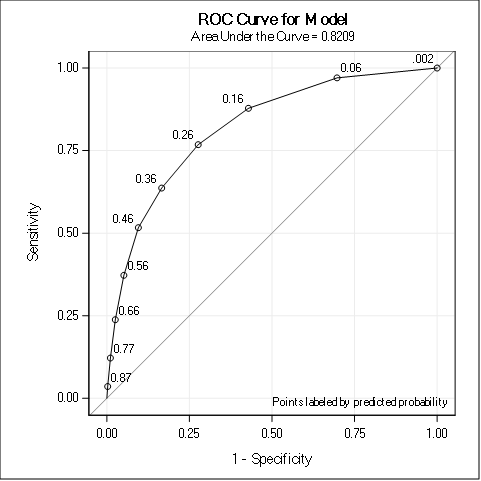
\includegraphics[height=3.54167in]{images/roc_s.png}

The ROC curve suggests that Model\_LogR\_S has 0.8209 coverage and lies
significantly above the diagonal. This is a slight improvement over the
ROC curve for Model\_LogR\_F.

\section{6 Model Selection}\label{model-selection}

The subjective model resulted in a specification with the highest AIC
score. This specification included 13 numeric variables which were hand
picked, however, a few of these variables were found to have
questionable polarity estimates. The forward selection technique
resulted in a specification with the lowest AIC score. However, this
specification included a number of insignificant variables. Finally, the
stepwise selection technique resulted in a specification with an AIC
only slightly higher than the forward selection technique, but avoided
including the high number of insignificant numeric variables.

A summary of performance metrics over each model using the training set
of data is shown below.

\paragraph{Table 6.1: Model Performance Metric
Summary}\label{table-6.1-model-performance-metric-summary}

\begin{longtable}[]{@{}lllllll@{}}
\toprule
Model & Pred & AIC & SC & KS & Ksa & ROC Coverage\tabularnewline
\midrule
\endhead
Model\_LogR\_Subj & 28 & 7003.854 & 7205.129 & 0.203568 & 17.787425 &
0.7993\tabularnewline
Model\_LogR\_F & 41 & 6722.759 & 7014.26 & 0.219433 & 19.173695 &
0.8202\tabularnewline
Model\_LogR\_S & 35 & 6726.476 & 6976.334 & 0.218525 & 19.094351 &
0.8209\tabularnewline
\bottomrule
\end{longtable}

Based on the results above, this assessment concludes that
Model\_LogR\_S is the superior model. Its performance metrics were among
the most favorable, yet it avoided the inclusion of insignificant
variables.

\section{7 Model Deployment Code}\label{model-deployment-code}

Please see Appendix A for the final deployment code.

\section{8 Bonus}\label{bonus}

Please see Appendix B for the coded decision tree.

\section{9 Conclusion}\label{conclusion}

Each of the logistic regression models fitted as part of this assessment
has its own definition of a `best' model specification. However this
assessment ultimately found Model\_LogR\_S to be the superior model for
predicting the probability of an accident, due to its relatively low AIC
score and since it retained only significant variables. It is important
to note however, that no single statistical method can be relied on to
identify the `true' or `best' model. Effective model building requires
substantive theory to suggest relevant predictors and plausible
functional forms for the model. This may be particularly relevant when
considering the short-comings of the dataset used for this assessment.
That is, we found little statistical relationship between many of the
variables within the dataset, yet, we had a fundamental basis for
including many variables and an expectation of appropriate coefficient
polarity and model specification based on those fundamentals.

\newpage

\section{Appendix A: Final Deployment
Code}\label{appendix-a-final-deployment-code}

\begin{Shaded}
\begin{Highlighting}[]

\NormalTok{%LET key }\KeywordTok{=} \KeywordTok{INDEX}\NormalTok{;}
\NormalTok{%LET response1 }\KeywordTok{=} \NormalTok{TARGET_FLAG;}
\NormalTok{%LET response2 }\KeywordTok{=} \NormalTok{TARGET_AMT;}
\NormalTok{%LET varname }\KeywordTok{=} \NormalTok{name;}

\NormalTok{%LET data }\KeywordTok{=} \NormalTok{logit_insurance;}
\NormalTok{%LET contents }\KeywordTok{=} \KeywordTok{&}\NormalTok{data._contents;}


\CommentTok{* Load the dataset;}

\NormalTok{libname mydata }\StringTok{'/sscc/home/d/dgb2583/411/'} \FunctionTok{access} \KeywordTok{=} \NormalTok{readonly;}

\DataTypeTok{DATA} \KeywordTok{&}\NormalTok{data.;}
    \KeywordTok{*}\NormalTok{SET mydata.logit_insurance;}
    \NormalTok{SET mydata.logit_insurance_test;}
\NormalTok{RUN; QUIT;}

\NormalTok{PROC CONTENTS DATA }\KeywordTok{=} \KeywordTok{&}\NormalTok{data. OUT }\KeywordTok{=} \KeywordTok{&}\NormalTok{contents.;}
\NormalTok{RUN; QUIT;}

\CommentTok{*PROC PRINT DATA = &contents. (OBS=20);}
\CommentTok{*RUN; QUIT;}

\NormalTok{PROC MEANS DATA }\KeywordTok{=} \KeywordTok{&}\NormalTok{data. }\KeywordTok{MIN} \NormalTok{P5 P50 P90 P95 P99 }\KeywordTok{MAX} \NormalTok{MEAN STDDEV NMISS N;}
\NormalTok{RUN; QUIT;}


\CommentTok{* Data rename;}

\NormalTok{%MACRO rename_num(varname);}
\DataTypeTok{    DATA} \KeywordTok{&}\NormalTok{data_def.;}
        \NormalTok{SET }\KeywordTok{&}\NormalTok{data_def. (RENAME }\KeywordTok{=} \NormalTok{(}\KeywordTok{&}\NormalTok{varname. }\KeywordTok{=} \NormalTok{N_}\KeywordTok{&}\NormalTok{varname.));}
    \NormalTok{RUN; QUIT;}
\NormalTok{%MEND;}

\NormalTok{%MACRO rename_cat(varname);}
\DataTypeTok{    DATA} \KeywordTok{&}\NormalTok{data_def.;}
        \NormalTok{SET }\KeywordTok{&}\NormalTok{data_def. (RENAME }\KeywordTok{=} \NormalTok{(}\KeywordTok{&}\NormalTok{varname. }\KeywordTok{=} \NormalTok{C_}\KeywordTok{&}\NormalTok{varname.));}
    \NormalTok{RUN; QUIT;}
\NormalTok{%MEND;}

\NormalTok{TITLE1 }\StringTok{''}\NormalTok{;}
\NormalTok{TITLE2 }\StringTok{''}\NormalTok{;}

\DataTypeTok{DATA} \KeywordTok{&}\NormalTok{data._name;}
    \NormalTok{SET }\KeywordTok{&}\NormalTok{data.;}
\NormalTok{RUN; QUIT;}

\NormalTok{PROC CONTENTS DATA }\KeywordTok{=} \KeywordTok{&}\NormalTok{data._name OUT }\KeywordTok{=} \KeywordTok{&}\NormalTok{contents._name;}
\NormalTok{RUN; QUIT;}

\DataTypeTok{DATA} \KeywordTok{&}\NormalTok{contents._name;}
    \NormalTok{SET }\KeywordTok{&}\NormalTok{contents._name;}
        \KeywordTok{IF} \NormalTok{name }\KeywordTok{=} \StringTok{"&key."} \KeywordTok{then} \NormalTok{DELETE;}
        \KeywordTok{IF} \NormalTok{name }\KeywordTok{=} \StringTok{"&response1."} \KeywordTok{then} \NormalTok{DELETE;}
        \KeywordTok{IF} \NormalTok{name }\KeywordTok{=} \StringTok{"&response2."} \KeywordTok{then} \NormalTok{DELETE;}
\NormalTok{RUN; QUIT;}

\NormalTok{%LET data_def }\KeywordTok{=} \KeywordTok{&}\NormalTok{data._name;}

\DataTypeTok{DATA} \NormalTok{_null_;}
    \KeywordTok{DO} \NormalTok{i }\KeywordTok{=} \DecValTok{1} \KeywordTok{to} \NormalTok{NUM;}
        \NormalTok{SET }\KeywordTok{&}\NormalTok{contents._name NOBS }\KeywordTok{=} \NormalTok{NUM;}
            \KeywordTok{WHERE} \DataTypeTok{type} \KeywordTok{=} \DecValTok{1}\NormalTok{;}
                \KeywordTok{CALL} \NormalTok{EXECUTE(}\StringTok{'%rename_num('}\KeywordTok{||}\NormalTok{name}\KeywordTok{||}\StringTok{')'}\NormalTok{);}
    \KeywordTok{END}\NormalTok{;}
\NormalTok{RUN; QUIT;}

\DataTypeTok{DATA} \NormalTok{_null_;}
    \KeywordTok{DO} \NormalTok{i }\KeywordTok{=} \DecValTok{1} \KeywordTok{to} \NormalTok{NUM;}
        \NormalTok{SET }\KeywordTok{&}\NormalTok{contents._name NOBS }\KeywordTok{=} \NormalTok{NUM;}
            \KeywordTok{WHERE} \DataTypeTok{type} \KeywordTok{=} \DecValTok{2}\NormalTok{;}
                \KeywordTok{CALL} \NormalTok{EXECUTE(}\StringTok{'%rename_cat('}\KeywordTok{||}\NormalTok{name}\KeywordTok{||}\StringTok{')'}\NormalTok{);}
    \KeywordTok{END}\NormalTok{;}
\NormalTok{RUN; QUIT;}

\DataTypeTok{DATA} \KeywordTok{&}\NormalTok{data._name;}
    \NormalTok{SET }\KeywordTok{&}\NormalTok{data._name;}
    \KeywordTok{IF} \NormalTok{C_EDUCATION }\KeywordTok{=} \StringTok{"<High School"}             \KeywordTok{then} \NormalTok{C_EDUCATION }\KeywordTok{=} \StringTok{"LT_HS"}\NormalTok{;}
    \KeywordTok{IF} \NormalTok{C_EDUCATION }\KeywordTok{=} \StringTok{"z_High School"}            \KeywordTok{then} \NormalTok{C_EDUCATION }\KeywordTok{=} \StringTok{"z_HS"}\NormalTok{;}
    \KeywordTok{IF} \NormalTok{C_JOB }\KeywordTok{=} \StringTok{"z_Blue Collar"}                  \KeywordTok{then} \NormalTok{C_JOB }\KeywordTok{=} \StringTok{"z_BC"}\NormalTok{;}
    \KeywordTok{IF} \NormalTok{C_JOB }\KeywordTok{=} \StringTok{"Home Maker"}                     \KeywordTok{then} \NormalTok{C_JOB }\KeywordTok{=} \StringTok{"Home_Maker"}\NormalTok{;}
    \KeywordTok{IF} \NormalTok{C_CAR_TYPE }\KeywordTok{=} \StringTok{"Panel Truck"}               \KeywordTok{then} \NormalTok{C_CAR_TYPE }\KeywordTok{=} \StringTok{"Panel_Truck"}\NormalTok{;}
    \KeywordTok{IF} \NormalTok{C_CAR_TYPE }\KeywordTok{=} \StringTok{"Sports Car"}                \KeywordTok{then} \NormalTok{C_CAR_TYPE }\KeywordTok{=} \StringTok{"Sports_Car"}\NormalTok{;}
    \KeywordTok{IF} \NormalTok{C_RED_CAR }\KeywordTok{=} \StringTok{"no"}                         \KeywordTok{then} \NormalTok{C_RED_CAR }\KeywordTok{=} \StringTok{"No"}\NormalTok{;}
    \KeywordTok{IF} \NormalTok{C_RED_CAR }\KeywordTok{=} \StringTok{"yes"}                        \KeywordTok{then} \NormalTok{C_RED_CAR }\KeywordTok{=} \StringTok{"Yes"}\NormalTok{;}
    \KeywordTok{IF} \NormalTok{C_URBANICITY }\KeywordTok{=} \StringTok{"Highly Urban/ Urban"}     \KeywordTok{then} \NormalTok{C_URBANICITY }\KeywordTok{=} \StringTok{"Urban"}\NormalTok{;}
    \KeywordTok{IF} \NormalTok{C_URBANICITY }\KeywordTok{=} \StringTok{"z_Highly Rural/ Rural"}   \KeywordTok{then} \NormalTok{C_URBANICITY }\KeywordTok{=} \StringTok{"z_Rural"}\NormalTok{;}
\NormalTok{RUN; QUIT;}

\NormalTok{PROC MEANS DATA }\KeywordTok{=} \KeywordTok{&}\NormalTok{data._name }\KeywordTok{MIN} \NormalTok{P5 P50 P90 P95 P99 }\KeywordTok{MAX} \NormalTok{MEAN STDDEV NMISS N;}
\NormalTok{RUN; QUIT;}

\NormalTok{PROC CONTENTS DATA }\KeywordTok{=} \KeywordTok{&}\NormalTok{data._name OUT }\KeywordTok{=} \KeywordTok{&}\NormalTok{contents._name;}
\NormalTok{RUN; QUIT;}


\CommentTok{* Data preparation;}

\NormalTok{%MACRO means(varname);}
    \NormalTok{PROC means DATA }\KeywordTok{=} \KeywordTok{&}\NormalTok{data_def. noprint;}
    \NormalTok{OUTPUT OUT }\KeywordTok{=} \KeywordTok{&}\NormalTok{varname. (DROP }\KeywordTok{=} \NormalTok{_freq_ _type_)}
        \NormalTok{nmiss(}\KeywordTok{&}\NormalTok{varname.)    }\KeywordTok{=} \KeywordTok{&}\NormalTok{varname._nmiss}
        \NormalTok{n(}\KeywordTok{&}\NormalTok{varname.)        }\KeywordTok{=} \KeywordTok{&}\NormalTok{varname._n}
        \NormalTok{mean(}\KeywordTok{&}\NormalTok{varname.)     }\KeywordTok{=} \KeywordTok{&}\NormalTok{varname._mean}
        \NormalTok{median(}\KeywordTok{&}\NormalTok{varname.)   }\KeywordTok{=} \KeywordTok{&}\NormalTok{varname._median}
        \NormalTok{mode(}\KeywordTok{&}\NormalTok{varname.)     }\KeywordTok{=} \KeywordTok{&}\NormalTok{varname._mode}
        \NormalTok{std(}\KeywordTok{&}\NormalTok{varname.)      }\KeywordTok{=} \KeywordTok{&}\NormalTok{varname._std}
        \NormalTok{skew(}\KeywordTok{&}\NormalTok{varname.)     }\KeywordTok{=} \KeywordTok{&}\NormalTok{varname._skew}
        \NormalTok{P1(}\KeywordTok{&}\NormalTok{varname.)       }\KeywordTok{=} \KeywordTok{&}\NormalTok{varname._P1}
        \NormalTok{P5(}\KeywordTok{&}\NormalTok{varname.)       }\KeywordTok{=} \KeywordTok{&}\NormalTok{varname._P5}
        \NormalTok{P10(}\KeywordTok{&}\NormalTok{varname.)      }\KeywordTok{=} \KeywordTok{&}\NormalTok{varname._P10}
        \NormalTok{P25(}\KeywordTok{&}\NormalTok{varname.)      }\KeywordTok{=} \KeywordTok{&}\NormalTok{varname._P25}
        \NormalTok{P50(}\KeywordTok{&}\NormalTok{varname.)      }\KeywordTok{=} \KeywordTok{&}\NormalTok{varname._P50}
        \NormalTok{P75(}\KeywordTok{&}\NormalTok{varname.)      }\KeywordTok{=} \KeywordTok{&}\NormalTok{varname._P75}
        \NormalTok{P90(}\KeywordTok{&}\NormalTok{varname.)      }\KeywordTok{=} \KeywordTok{&}\NormalTok{varname._P90}
        \NormalTok{P95(}\KeywordTok{&}\NormalTok{varname.)      }\KeywordTok{=} \KeywordTok{&}\NormalTok{varname._P95}
        \NormalTok{P99(}\KeywordTok{&}\NormalTok{varname.)      }\KeywordTok{=} \KeywordTok{&}\NormalTok{varname._P99}
        \KeywordTok{min}\NormalTok{(}\KeywordTok{&}\NormalTok{varname.)      }\KeywordTok{=} \KeywordTok{&}\NormalTok{varname._min}
        \KeywordTok{max}\NormalTok{(}\KeywordTok{&}\NormalTok{varname.)      }\KeywordTok{=} \KeywordTok{&}\NormalTok{varname._max}
        \NormalTok{qrange(}\KeywordTok{&}\NormalTok{varname.)   }\KeywordTok{=} \KeywordTok{&}\NormalTok{varname._qrange}
        \NormalTok{;}
    \NormalTok{RUN; QUIT;}
\NormalTok{%MEND;}

\NormalTok{%MACRO }\FunctionTok{transpose}\NormalTok{(varname);}
    \NormalTok{PROC }\FunctionTok{transpose} \NormalTok{DATA }\KeywordTok{=} \KeywordTok{&}\NormalTok{varname. OUT }\KeywordTok{=} \KeywordTok{&}\NormalTok{varname._t;}
        \NormalTok{var _numeric_;}
    \NormalTok{RUN; QUIT;}
\NormalTok{%MEND;}

\NormalTok{%MACRO symputx_num(varname);}
\DataTypeTok{    DATA} \NormalTok{_null_;}
        \NormalTok{SET }\KeywordTok{&}\NormalTok{varname._t;}
            \KeywordTok{CALL} \NormalTok{symputx(_name_, strip(col1), }\StringTok{'g'}\NormalTok{);}
    \NormalTok{RUN; QUIT;}
\NormalTok{%MEND;}

\NormalTok{%MACRO outlier(varname);}
\DataTypeTok{    DATA} \KeywordTok{&}\NormalTok{data_def.;}
        \NormalTok{SET }\KeywordTok{&}\NormalTok{data_def.;}
            \KeywordTok{*IF} \NormalTok{(}\KeywordTok{&}\NormalTok{varname. }\KeywordTok{<} \KeywordTok{&&&}\NormalTok{varname._P10) OR (}\KeywordTok{&}\NormalTok{varname. }\KeywordTok{>} \KeywordTok{&&&}\NormalTok{varname._P90) }\KeywordTok{THEN}
            \KeywordTok{*}   \KeywordTok{&}\NormalTok{varname._OF }\KeywordTok{=} \FloatTok{1.0}\NormalTok{; }\KeywordTok{*ELSE} \KeywordTok{&}\NormalTok{varname._OF }\KeywordTok{=} \FloatTok{0.0}\NormalTok{;}
            
            \KeywordTok{*IF} \NormalTok{(}\KeywordTok{&}\NormalTok{varname. }\KeywordTok{<} \KeywordTok{&&&}\NormalTok{varname._P5) OR (}\KeywordTok{&}\NormalTok{varname. }\KeywordTok{>} \KeywordTok{&&&}\NormalTok{varname._P95) }\KeywordTok{THEN}
            \KeywordTok{*}   \KeywordTok{&}\NormalTok{varname._OF }\KeywordTok{=} \FloatTok{1.0}\NormalTok{; }\KeywordTok{*ELSE} \KeywordTok{&}\NormalTok{varname._OF }\KeywordTok{=} \FloatTok{0.0}\NormalTok{;}
            
            \KeywordTok{IF} \NormalTok{(}\KeywordTok{&}\NormalTok{varname. }\KeywordTok{<} \KeywordTok{&&&}\NormalTok{varname._P1) OR (}\KeywordTok{&}\NormalTok{varname. }\KeywordTok{>} \KeywordTok{&&&}\NormalTok{varname._P99) }\KeywordTok{THEN}
                \KeywordTok{&}\NormalTok{varname._OF }\KeywordTok{=} \FloatTok{1.0}\NormalTok{; }\KeywordTok{ELSE} \KeywordTok{&}\NormalTok{varname._OF }\KeywordTok{=} \FloatTok{0.0}\NormalTok{;}
    \NormalTok{RUN; QUIT;}
\NormalTok{%MEND;}

\NormalTok{%MACRO }\FunctionTok{trim}\NormalTok{(varname);}
\DataTypeTok{    DATA} \KeywordTok{&}\NormalTok{data_def.;}
        \NormalTok{SET }\KeywordTok{&}\NormalTok{data_def.;}
            \KeywordTok{&}\NormalTok{varname._T90 }\KeywordTok{=} \KeywordTok{&}\NormalTok{varname.;}
            \KeywordTok{*&}\NormalTok{varname._T90 }\KeywordTok{=} \KeywordTok{max}\NormalTok{(}\KeywordTok{min}\NormalTok{(}\KeywordTok{&}\NormalTok{varname.,}\KeywordTok{&&&}\NormalTok{varname._P90),}\KeywordTok{&&&}\NormalTok{varname._P10);}
            \KeywordTok{IF} \NormalTok{(}\KeywordTok{&}\NormalTok{varname._T90 }\KeywordTok{<} \KeywordTok{&&&}\NormalTok{varname._P10) OR (}\KeywordTok{&}\NormalTok{varname._T99 }\KeywordTok{>} \KeywordTok{&&&}\NormalTok{varname._P90) }\KeywordTok{THEN}
                \KeywordTok{&}\NormalTok{varname._T90 }\KeywordTok{=} \StringTok{'.'}\NormalTok{;}
            
            \KeywordTok{*&}\NormalTok{varname._T95 }\KeywordTok{=} \KeywordTok{&}\NormalTok{varname.;}
            \KeywordTok{*&}\NormalTok{varname._T95 }\KeywordTok{=} \KeywordTok{max}\NormalTok{(}\KeywordTok{min}\NormalTok{(}\KeywordTok{&}\NormalTok{varname.,}\KeywordTok{&&&}\NormalTok{varname._P95),}\KeywordTok{&&&}\NormalTok{varname._P5);}
            \KeywordTok{*IF} \NormalTok{(}\KeywordTok{&}\NormalTok{varname._T95 }\KeywordTok{<} \KeywordTok{&&&}\NormalTok{varname._P5) OR (}\KeywordTok{&}\NormalTok{varname._T95 }\KeywordTok{>} \KeywordTok{&&&}\NormalTok{varname._P95) }\KeywordTok{THEN}
            \KeywordTok{*}   \KeywordTok{&}\NormalTok{varname._T95 }\KeywordTok{=} \StringTok{'.'}\NormalTok{;}
            
            \KeywordTok{&}\NormalTok{varname._T99 }\KeywordTok{=} \KeywordTok{&}\NormalTok{varname.;}
            \KeywordTok{*&}\NormalTok{varname._T99 }\KeywordTok{=} \KeywordTok{max}\NormalTok{(}\KeywordTok{min}\NormalTok{(}\KeywordTok{&}\NormalTok{varname.,}\KeywordTok{&&&}\NormalTok{varname._P99),}\KeywordTok{&&&}\NormalTok{varname._P1);}
            \KeywordTok{IF} \NormalTok{(}\KeywordTok{&}\NormalTok{varname._T99 }\KeywordTok{<} \KeywordTok{&&&}\NormalTok{varname._P1) OR (}\KeywordTok{&}\NormalTok{varname._T99 }\KeywordTok{>} \KeywordTok{&&&}\NormalTok{varname._P99) }\KeywordTok{THEN}
                \KeywordTok{&}\NormalTok{varname._T99 }\KeywordTok{=} \StringTok{'.'}\NormalTok{;}
    \NormalTok{RUN; QUIT;}
\NormalTok{%MEND;}

\NormalTok{%MACRO missing(varname);}
\DataTypeTok{    DATA} \KeywordTok{&}\NormalTok{data_def.;}
        \NormalTok{SET }\KeywordTok{&}\NormalTok{data_def.;}
            \KeywordTok{IF} \NormalTok{missing(}\KeywordTok{&}\NormalTok{varname.) }\KeywordTok{THEN}
                \KeywordTok{&}\NormalTok{varname._MF }\KeywordTok{=} \FloatTok{1.0}\NormalTok{; }\KeywordTok{ELSE} \KeywordTok{&}\NormalTok{varname._MF }\KeywordTok{=} \FloatTok{0.0}\NormalTok{;}
    \NormalTok{RUN; QUIT;}
\NormalTok{%MEND;}

\NormalTok{%MACRO impute(varname);}
\DataTypeTok{    DATA} \KeywordTok{&}\NormalTok{data_def.;}
        \NormalTok{SET }\KeywordTok{&}\NormalTok{data_def.;}
            \KeywordTok{*&}\NormalTok{varname._IMU }\KeywordTok{=} \KeywordTok{&}\NormalTok{varname.;}
            \KeywordTok{*IF} \NormalTok{missing(}\KeywordTok{&}\NormalTok{varname._IMU) }\KeywordTok{THEN}
            \KeywordTok{*}   \KeywordTok{&}\NormalTok{varname._IMU }\KeywordTok{=} \KeywordTok{&&&}\NormalTok{varname._mean;}
            
            \KeywordTok{*&}\NormalTok{varname._IMO }\KeywordTok{=} \KeywordTok{&}\NormalTok{varname.;}
            \KeywordTok{*IF} \NormalTok{missing(}\KeywordTok{&}\NormalTok{varname._IMO) }\KeywordTok{THEN}
            \KeywordTok{*}   \KeywordTok{&}\NormalTok{varname._IMO }\KeywordTok{=} \KeywordTok{&&&}\NormalTok{varname._mode;}
            
            \KeywordTok{&}\NormalTok{varname._IME }\KeywordTok{=} \KeywordTok{&}\NormalTok{varname.;}
            \KeywordTok{IF} \NormalTok{missing(}\KeywordTok{&}\NormalTok{varname._IME) }\KeywordTok{THEN}
                \KeywordTok{&}\NormalTok{varname._IME }\KeywordTok{=} \KeywordTok{&&&}\NormalTok{varname._median;}
    \NormalTok{RUN; QUIT;}
\NormalTok{%MEND;}

\NormalTok{%MACRO transform(varname);}
\DataTypeTok{    DATA} \KeywordTok{&}\NormalTok{data_def.;}
        \NormalTok{SET }\KeywordTok{&}\NormalTok{data_def.;}
            \KeywordTok{&}\NormalTok{varname._LN }\KeywordTok{=} \KeywordTok{sign}\NormalTok{(}\KeywordTok{&}\NormalTok{varname.) }\KeywordTok{*} \KeywordTok{log}\NormalTok{(}\KeywordTok{abs}\NormalTok{(}\KeywordTok{&}\NormalTok{varname.)}\KeywordTok{+}\DecValTok{1}\NormalTok{);}
            \KeywordTok{*&}\NormalTok{varname._SQ }\KeywordTok{=} \NormalTok{(}\KeywordTok{&}\NormalTok{varname.}\KeywordTok{*&}\NormalTok{varname.);}
            \KeywordTok{*&}\NormalTok{varname._RT }\KeywordTok{=} \KeywordTok{sqrt}\NormalTok{(}\KeywordTok{&}\NormalTok{varname.);}
    \NormalTok{RUN; QUIT;}
\NormalTok{%MEND;}

\NormalTok{%MACRO drop(varname);}
\DataTypeTok{    DATA} \KeywordTok{&}\NormalTok{data_def.;}
        \NormalTok{SET }\KeywordTok{&}\NormalTok{data_def.;}
            \NormalTok{DROP }\KeywordTok{&}\NormalTok{varname.;}
    \NormalTok{RUN; QUIT;}
\NormalTok{%MEND;}

\NormalTok{TITLE1 }\StringTok{''}\NormalTok{;}
\NormalTok{TITLE2 }\StringTok{''}\NormalTok{;}

\CommentTok{* Adhoc changes;}

\DataTypeTok{DATA} \KeywordTok{&}\NormalTok{data._clean;}
    \NormalTok{SET }\KeywordTok{&}\NormalTok{data._name;}
\NormalTok{RUN; QUIT;}

\DataTypeTok{DATA} \KeywordTok{&}\NormalTok{data._clean;}
    \NormalTok{SET }\KeywordTok{&}\NormalTok{data._clean;}
    \NormalTok{N_CAR_AGE }\KeywordTok{=} \KeywordTok{abs}\NormalTok{(N_CAR_AGE);}
\NormalTok{RUN; QUIT;}

\CommentTok{* Create new dataset of flags for continuous variables;}

\DataTypeTok{DATA} \KeywordTok{&}\NormalTok{data._flag;}
    \NormalTok{SET }\KeywordTok{&}\NormalTok{data._clean;}
\NormalTok{RUN; QUIT;}

\NormalTok{PROC CONTENTS DATA }\KeywordTok{=} \KeywordTok{&}\NormalTok{data._flag OUT }\KeywordTok{=} \KeywordTok{&}\NormalTok{contents._flag;}
\NormalTok{RUN; QUIT;}

\DataTypeTok{DATA} \KeywordTok{&}\NormalTok{contents._flag;}
    \NormalTok{SET }\KeywordTok{&}\NormalTok{contents._flag;}
        \KeywordTok{IF} \NormalTok{name }\KeywordTok{=} \StringTok{"&key."} \KeywordTok{then} \NormalTok{DELETE;}
        \KeywordTok{IF} \NormalTok{name }\KeywordTok{=} \StringTok{"&response1."} \KeywordTok{then} \NormalTok{DELETE;}
        \KeywordTok{IF} \NormalTok{name }\KeywordTok{=} \StringTok{"&response2."} \KeywordTok{then} \NormalTok{DELETE;}
\NormalTok{RUN; QUIT;}

\NormalTok{%LET data_def }\KeywordTok{=} \KeywordTok{&}\NormalTok{data._flag;}

\DataTypeTok{DATA} \NormalTok{_null_;}
    \KeywordTok{DO} \NormalTok{i }\KeywordTok{=} \DecValTok{1} \KeywordTok{to} \NormalTok{NUM;}
        \NormalTok{SET }\KeywordTok{&}\NormalTok{contents._flag NOBS }\KeywordTok{=} \NormalTok{NUM;}
            \KeywordTok{WHERE} \DataTypeTok{type} \KeywordTok{=} \DecValTok{1}\NormalTok{;}
                \KeywordTok{CALL} \NormalTok{EXECUTE(}\StringTok{'%means('}\KeywordTok{||}\NormalTok{name}\KeywordTok{||}\StringTok{')'}\NormalTok{);}
                \KeywordTok{CALL} \NormalTok{EXECUTE(}\StringTok{'%transpose('}\KeywordTok{||}\NormalTok{name}\KeywordTok{||}\StringTok{')'}\NormalTok{);}
                \KeywordTok{CALL} \NormalTok{EXECUTE(}\StringTok{'%symputx_num('}\KeywordTok{||}\NormalTok{name}\KeywordTok{||}\StringTok{')'}\NormalTok{);}
    \KeywordTok{END}\NormalTok{;}
\NormalTok{RUN; QUIT;}

\DataTypeTok{DATA} \NormalTok{_null_;}
    \KeywordTok{DO} \NormalTok{i }\KeywordTok{=} \DecValTok{1} \KeywordTok{to} \NormalTok{NUM;}
        \NormalTok{SET }\KeywordTok{&}\NormalTok{contents._flag NOBS }\KeywordTok{=} \NormalTok{NUM;}
            \KeywordTok{WHERE} \DataTypeTok{type} \KeywordTok{=} \DecValTok{1}\NormalTok{;}
                \KeywordTok{CALL} \NormalTok{EXECUTE(}\StringTok{'%missing('}\KeywordTok{||}\NormalTok{name}\KeywordTok{||}\StringTok{')'}\NormalTok{);}
                \KeywordTok{CALL} \NormalTok{EXECUTE(}\StringTok{'%outlier('}\KeywordTok{||}\NormalTok{name}\KeywordTok{||}\StringTok{')'}\NormalTok{);}
    \KeywordTok{END}\NormalTok{;}
\NormalTok{RUN; QUIT;}

\DataTypeTok{DATA} \NormalTok{_null_;}
    \KeywordTok{DO} \NormalTok{i }\KeywordTok{=} \DecValTok{1} \KeywordTok{to} \NormalTok{NUM;}
        \NormalTok{SET }\KeywordTok{&}\NormalTok{contents._name NOBS }\KeywordTok{=} \NormalTok{NUM;}
            \KeywordTok{CALL} \NormalTok{EXECUTE(}\StringTok{'%drop('}\KeywordTok{||}\NormalTok{name}\KeywordTok{||}\StringTok{')'}\NormalTok{);}
    \KeywordTok{END}\NormalTok{;}
\NormalTok{RUN; QUIT;}

\DataTypeTok{DATA} \KeywordTok{&}\NormalTok{data._flag;}
    \KeywordTok{MERGE} \KeywordTok{&}\NormalTok{data._flag }\KeywordTok{&}\NormalTok{data.(KEEP }\KeywordTok{=} \KeywordTok{&}\NormalTok{key.);}
\NormalTok{RUN; QUIT;}

\NormalTok{PROC MEANS DATA }\KeywordTok{=} \KeywordTok{&}\NormalTok{data._flag }\KeywordTok{MIN} \NormalTok{P5 P50 P90 P95 P99 }\KeywordTok{MAX} \NormalTok{MEAN STDDEV NMISS N;}
\NormalTok{RUN; QUIT;}

\NormalTok{PROC CONTENTS DATA }\KeywordTok{=} \KeywordTok{&}\NormalTok{data._flag OUT }\KeywordTok{=} \KeywordTok{&}\NormalTok{contents._flag;}
\NormalTok{RUN; QUIT;}

\CommentTok{* Create dummy variables;}

\DataTypeTok{DATA} \KeywordTok{&}\NormalTok{data._dum;}
    \NormalTok{SET }\KeywordTok{&}\NormalTok{data._clean;}
\NormalTok{RUN; QUIT;}

\NormalTok{PROC CONTENTS DATA }\KeywordTok{=} \KeywordTok{&}\NormalTok{data._dum OUT }\KeywordTok{=} \KeywordTok{&}\NormalTok{contents._dum;}
\NormalTok{RUN; QUIT;}

\DataTypeTok{DATA} \KeywordTok{&}\NormalTok{contents._dum;}
    \NormalTok{SET }\KeywordTok{&}\NormalTok{contents._dum;}
        \KeywordTok{IF} \NormalTok{name }\KeywordTok{=} \StringTok{"&key."} \KeywordTok{then} \NormalTok{DELETE;}
        \KeywordTok{IF} \NormalTok{name }\KeywordTok{=} \StringTok{"&response1."} \KeywordTok{then} \NormalTok{DELETE;}
        \KeywordTok{IF} \NormalTok{name }\KeywordTok{=} \StringTok{"&response2."} \KeywordTok{then} \NormalTok{DELETE;}
\NormalTok{RUN; QUIT;}

\DataTypeTok{DATA} \KeywordTok{&}\NormalTok{data._dum;}
    \NormalTok{SET }\KeywordTok{&}\NormalTok{data._dum; }
        \NormalTok{N_AGE_Risk_Yes  }\KeywordTok{=}   \NormalTok{(N_AGE }\KeywordTok{<=} \DecValTok{30} \KeywordTok{|} \NormalTok{N_AGE }\KeywordTok{>=} \DecValTok{60}\NormalTok{);}
        \NormalTok{N_AGE_Risk_No   }\KeywordTok{=}   \NormalTok{(N_AGE_Risk_Yes }\KeywordTok{=} \DecValTok{0}\NormalTok{);}
        
        \NormalTok{N_BLUEBOOK_Hi   }\KeywordTok{=}   \NormalTok{(N_BLUEBOOK }\KeywordTok{>=} \DecValTok{27000}\NormalTok{);}
        \NormalTok{N_BLUEBOOK_Lo   }\KeywordTok{=}   \NormalTok{(N_BLUEBOOK_Hi }\KeywordTok{=} \DecValTok{0}\NormalTok{);}
        
        \NormalTok{N_CLM_FREQ_No   }\KeywordTok{=}   \NormalTok{(N_CLM_FREQ }\KeywordTok{=} \DecValTok{0}\NormalTok{);}
        \NormalTok{N_CLM_FREQ_Yes  }\KeywordTok{=}   \NormalTok{(N_CLM_FREQ }\KeywordTok{>} \DecValTok{0}\NormalTok{);}
        \NormalTok{N_CLM_FREQ_Hi   }\KeywordTok{=}   \NormalTok{(N_CLM_FREQ }\KeywordTok{>=} \DecValTok{2}\NormalTok{);}
        \NormalTok{N_CLM_FREQ_Lo   }\KeywordTok{=}   \NormalTok{(N_CLM_FREQ_Hi }\KeywordTok{=} \DecValTok{0}\NormalTok{);}

        \NormalTok{N_HOMEKIDS_No   }\KeywordTok{=}   \NormalTok{(N_HOMEKIDS }\KeywordTok{=} \DecValTok{0}\NormalTok{);}
        \NormalTok{N_HOMEKIDS_Yes  }\KeywordTok{=}   \NormalTok{(N_HOMEKIDS }\KeywordTok{>} \DecValTok{0}\NormalTok{);}
        
        \NormalTok{N_INCOME_No     }\KeywordTok{=}   \NormalTok{(N_INCOME }\KeywordTok{=} \DecValTok{0}\NormalTok{);}
        \NormalTok{N_INCOME_Yes    }\KeywordTok{=}   \NormalTok{(N_INCOME }\KeywordTok{>} \DecValTok{0}\NormalTok{);}
        \NormalTok{N_INCOME_Hi     }\KeywordTok{=}   \NormalTok{(N_INCOME }\KeywordTok{>=} \DecValTok{85000}\NormalTok{);}
        \NormalTok{N_INCOME_Lo     }\KeywordTok{=}   \NormalTok{(N_INCOME_Hi }\KeywordTok{=} \DecValTok{0}\NormalTok{);}
        
        \NormalTok{N_KIDSDRIV_No   }\KeywordTok{=}   \NormalTok{(N_KIDSDRIV }\KeywordTok{=} \DecValTok{0}\NormalTok{);}
        \NormalTok{N_KIDSDRIV_Yes  }\KeywordTok{=}   \NormalTok{(N_KIDSDRIV }\KeywordTok{>} \DecValTok{0}\NormalTok{);}
        
        \NormalTok{N_MVR_PTS_No    }\KeywordTok{=}   \NormalTok{(N_MVR_PTS }\KeywordTok{=} \DecValTok{0}\NormalTok{);}
        \NormalTok{N_MVR_PTS_Yes   }\KeywordTok{=}   \NormalTok{(N_MVR_PTS }\KeywordTok{>} \DecValTok{0}\NormalTok{);}
        \NormalTok{N_MVR_PTS_Hi    }\KeywordTok{=}   \NormalTok{(N_MVR_PTS }\KeywordTok{>=} \DecValTok{4}\NormalTok{);}
        \NormalTok{N_MVR_PTS_Lo    }\KeywordTok{=}   \NormalTok{(N_MVR_PTS_Hi }\KeywordTok{=} \DecValTok{0}\NormalTok{);}
        
        \NormalTok{N_OLDCLAIM_No   }\KeywordTok{=}   \NormalTok{(N_OLDCLAIM }\KeywordTok{=} \DecValTok{0}\NormalTok{);}
        \NormalTok{N_OLDCLAIM_Yes  }\KeywordTok{=}   \NormalTok{(N_OLDCLAIM }\KeywordTok{>} \DecValTok{0}\NormalTok{);}
        \NormalTok{N_OLDCLAIM_Hi   }\KeywordTok{=}   \NormalTok{(N_OLDCLAIM }\KeywordTok{>=} \DecValTok{9500}\NormalTok{);}
        \NormalTok{N_OLDCLAIM_Lo   }\KeywordTok{=}   \NormalTok{(N_OLDCLAIM_Hi }\KeywordTok{=} \DecValTok{0}\NormalTok{);}
        
        \NormalTok{N_RENTER_Yes    }\KeywordTok{=}   \NormalTok{(N_HOME_VAL }\KeywordTok{<=} \DecValTok{14400}\NormalTok{);}
        \NormalTok{N_RENTER_No     }\KeywordTok{=}   \NormalTok{(N_RENTER_Yes }\KeywordTok{=} \DecValTok{0}\NormalTok{);}
        
        \NormalTok{N_TRAVTIME_Hi   }\KeywordTok{=}   \NormalTok{(N_TRAVTIME }\KeywordTok{>=} \DecValTok{50}\NormalTok{);}
        \NormalTok{N_TRAVTIME_Lo   }\KeywordTok{=}   \NormalTok{(N_TRAVTIME_Hi }\KeywordTok{=} \DecValTok{0}\NormalTok{);}
\NormalTok{RUN; QUIT;}

\NormalTok{%LET data_def }\KeywordTok{=} \KeywordTok{&}\NormalTok{data._dum;}

\DataTypeTok{DATA} \NormalTok{_null_;}
    \KeywordTok{DO} \NormalTok{i }\KeywordTok{=} \DecValTok{1} \KeywordTok{to} \NormalTok{NUM;}
        \NormalTok{SET }\KeywordTok{&}\NormalTok{contents._name NOBS }\KeywordTok{=} \NormalTok{NUM;}
            \KeywordTok{CALL} \NormalTok{EXECUTE(}\StringTok{'%drop('}\KeywordTok{||}\NormalTok{name}\KeywordTok{||}\StringTok{')'}\NormalTok{);}
    \KeywordTok{END}\NormalTok{;}
\NormalTok{RUN; QUIT;}

\DataTypeTok{DATA} \KeywordTok{&}\NormalTok{data._dum;}
    \KeywordTok{MERGE} \KeywordTok{&}\NormalTok{data._dum }\KeywordTok{&}\NormalTok{data.(KEEP }\KeywordTok{=} \KeywordTok{&}\NormalTok{key.);}
\NormalTok{RUN; QUIT;}

\NormalTok{PROC MEANS DATA }\KeywordTok{=} \KeywordTok{&}\NormalTok{data._dum }\KeywordTok{MIN} \NormalTok{P5 P50 P90 P95 P99 }\KeywordTok{MAX} \NormalTok{MEAN STDDEV NMISS N;}
\NormalTok{RUN; QUIT;}

\NormalTok{PROC CONTENTS DATA }\KeywordTok{=} \KeywordTok{&}\NormalTok{data._dum OUT }\KeywordTok{=} \KeywordTok{&}\NormalTok{contents._dum;}
\NormalTok{RUN; QUIT;}

\CommentTok{* Add trimmed series to original dataset;}

\DataTypeTok{DATA} \KeywordTok{&}\NormalTok{data._trim;}
    \NormalTok{SET }\KeywordTok{&}\NormalTok{data._clean;}
\NormalTok{RUN; QUIT;}

\NormalTok{PROC CONTENTS DATA }\KeywordTok{=} \KeywordTok{&}\NormalTok{data._trim OUT }\KeywordTok{=} \KeywordTok{&}\NormalTok{contents._trim;}
\NormalTok{RUN; QUIT;}

\DataTypeTok{DATA} \KeywordTok{&}\NormalTok{contents._trim;}
    \NormalTok{SET }\KeywordTok{&}\NormalTok{contents._trim;}
        \KeywordTok{IF} \NormalTok{name }\KeywordTok{=} \StringTok{"&key."} \KeywordTok{then} \NormalTok{DELETE;}
        \KeywordTok{IF} \NormalTok{name }\KeywordTok{=} \StringTok{"&response1."} \KeywordTok{then} \NormalTok{DELETE;}
        \KeywordTok{IF} \NormalTok{name }\KeywordTok{=} \StringTok{"&response2."} \KeywordTok{then} \NormalTok{DELETE;}
\NormalTok{RUN; QUIT;}

\NormalTok{%LET data_def }\KeywordTok{=} \KeywordTok{&}\NormalTok{data._trim;}

\DataTypeTok{DATA} \NormalTok{_null_;}
    \KeywordTok{DO} \NormalTok{i }\KeywordTok{=} \DecValTok{1} \KeywordTok{to} \NormalTok{NUM;}
        \NormalTok{SET }\KeywordTok{&}\NormalTok{contents._trim NOBS }\KeywordTok{=} \NormalTok{NUM;}
            \KeywordTok{WHERE} \DataTypeTok{type} \KeywordTok{=} \DecValTok{1}\NormalTok{;}
                \KeywordTok{CALL} \NormalTok{EXECUTE(}\StringTok{'%means('}\KeywordTok{||}\NormalTok{name}\KeywordTok{||}\StringTok{')'}\NormalTok{);}
                \KeywordTok{CALL} \NormalTok{EXECUTE(}\StringTok{'%transpose('}\KeywordTok{||}\NormalTok{name}\KeywordTok{||}\StringTok{')'}\NormalTok{);}
                \KeywordTok{CALL} \NormalTok{EXECUTE(}\StringTok{'%symputx_num('}\KeywordTok{||}\NormalTok{name}\KeywordTok{||}\StringTok{')'}\NormalTok{);}
    \KeywordTok{END}\NormalTok{;}
\NormalTok{RUN; QUIT;}

\DataTypeTok{DATA} \NormalTok{_null_;}
    \KeywordTok{DO} \NormalTok{i }\KeywordTok{=} \DecValTok{1} \KeywordTok{to} \NormalTok{NUM;}
        \NormalTok{SET }\KeywordTok{&}\NormalTok{contents._trim NOBS }\KeywordTok{=} \NormalTok{NUM;}
            \KeywordTok{WHERE} \DataTypeTok{type} \KeywordTok{=} \DecValTok{1}\NormalTok{;}
                \KeywordTok{CALL} \NormalTok{EXECUTE(}\StringTok{'%trim('}\KeywordTok{||}\NormalTok{name}\KeywordTok{||}\StringTok{')'}\NormalTok{);}
    \KeywordTok{END}\NormalTok{;}
\NormalTok{RUN; QUIT;}

\CommentTok{* Impute all continuous series in original dataset;}

\DataTypeTok{DATA} \KeywordTok{&}\NormalTok{data._imp;}
    \NormalTok{SET }\KeywordTok{&}\NormalTok{data._trim;}
\NormalTok{RUN; QUIT;}

\NormalTok{PROC CONTENTS DATA }\KeywordTok{=} \KeywordTok{&}\NormalTok{data._imp OUT }\KeywordTok{=} \KeywordTok{&}\NormalTok{contents._imp;}
\NormalTok{RUN; QUIT;}

\DataTypeTok{DATA} \KeywordTok{&}\NormalTok{contents._imp;}
    \NormalTok{SET }\KeywordTok{&}\NormalTok{contents._imp;}
        \KeywordTok{IF} \NormalTok{name }\KeywordTok{=} \StringTok{"&key."} \KeywordTok{then} \NormalTok{DELETE;}
        \KeywordTok{IF} \NormalTok{name }\KeywordTok{=} \StringTok{"&response1."} \KeywordTok{then} \NormalTok{DELETE;}
        \KeywordTok{IF} \NormalTok{name }\KeywordTok{=} \StringTok{"&response2."} \KeywordTok{then} \NormalTok{DELETE;}
\NormalTok{RUN; QUIT;}

\NormalTok{%LET data_def }\KeywordTok{=} \KeywordTok{&}\NormalTok{data._imp;}

\DataTypeTok{DATA} \NormalTok{_null_;}
    \KeywordTok{DO} \NormalTok{i }\KeywordTok{=} \DecValTok{1} \KeywordTok{to} \NormalTok{NUM;}
        \NormalTok{SET }\KeywordTok{&}\NormalTok{contents._imp NOBS }\KeywordTok{=} \NormalTok{NUM;}
            \KeywordTok{WHERE} \DataTypeTok{type} \KeywordTok{=} \DecValTok{1}\NormalTok{;}
                \KeywordTok{CALL} \NormalTok{EXECUTE(}\StringTok{'%means('}\KeywordTok{||}\NormalTok{name}\KeywordTok{||}\StringTok{')'}\NormalTok{);}
                \KeywordTok{CALL} \NormalTok{EXECUTE(}\StringTok{'%transpose('}\KeywordTok{||}\NormalTok{name}\KeywordTok{||}\StringTok{')'}\NormalTok{);}
                \KeywordTok{CALL} \NormalTok{EXECUTE(}\StringTok{'%symputx_num('}\KeywordTok{||}\NormalTok{name}\KeywordTok{||}\StringTok{')'}\NormalTok{);}
    \KeywordTok{END}\NormalTok{;}
\NormalTok{RUN; QUIT;}

\DataTypeTok{DATA} \NormalTok{_null_;}
    \KeywordTok{DO} \NormalTok{i }\KeywordTok{=} \DecValTok{1} \KeywordTok{to} \NormalTok{NUM;}
        \NormalTok{SET }\KeywordTok{&}\NormalTok{contents._imp NOBS }\KeywordTok{=} \NormalTok{NUM;}
            \KeywordTok{WHERE} \DataTypeTok{type} \KeywordTok{=} \DecValTok{1}\NormalTok{;}
                \KeywordTok{CALL} \NormalTok{EXECUTE(}\StringTok{'%impute('}\KeywordTok{||}\NormalTok{name}\KeywordTok{||}\StringTok{')'}\NormalTok{);}
    \KeywordTok{END}\NormalTok{;}
\NormalTok{RUN; QUIT;}

\DataTypeTok{DATA} \NormalTok{_null_;}
    \KeywordTok{DO} \NormalTok{i }\KeywordTok{=} \DecValTok{1} \KeywordTok{to} \NormalTok{NUM;}
        \NormalTok{SET }\KeywordTok{&}\NormalTok{contents._imp NOBS }\KeywordTok{=} \NormalTok{NUM;}
            \KeywordTok{WHERE} \DataTypeTok{type} \KeywordTok{=} \DecValTok{1}\NormalTok{;}
                \KeywordTok{CALL} \NormalTok{EXECUTE(}\StringTok{'%drop('}\KeywordTok{||}\NormalTok{name}\KeywordTok{||}\StringTok{')'}\NormalTok{);}
    \KeywordTok{END}\NormalTok{;}
\NormalTok{RUN; QUIT;}

\CommentTok{* Transform all continuous series in original dataset;}

\DataTypeTok{DATA} \KeywordTok{&}\NormalTok{data._trans;}
    \NormalTok{SET }\KeywordTok{&}\NormalTok{data._imp;}
\NormalTok{RUN; QUIT;}

\NormalTok{PROC CONTENTS DATA }\KeywordTok{=} \KeywordTok{&}\NormalTok{data._trans OUT }\KeywordTok{=} \KeywordTok{&}\NormalTok{contents._trans;}
\NormalTok{RUN; QUIT;}

\DataTypeTok{DATA} \KeywordTok{&}\NormalTok{contents._trans;}
    \NormalTok{SET }\KeywordTok{&}\NormalTok{contents._trans;}
        \KeywordTok{IF} \NormalTok{name }\KeywordTok{=} \StringTok{"&key."} \KeywordTok{then} \NormalTok{DELETE;}
        \KeywordTok{IF} \NormalTok{name }\KeywordTok{=} \StringTok{"&response1."} \KeywordTok{then} \NormalTok{DELETE;}
        \KeywordTok{IF} \NormalTok{name }\KeywordTok{=} \StringTok{"&response2."} \KeywordTok{then} \NormalTok{DELETE;}
\NormalTok{RUN; QUIT;}

\NormalTok{%LET data_def }\KeywordTok{=} \KeywordTok{&}\NormalTok{data._trans;}

\DataTypeTok{DATA} \NormalTok{_null_;}
    \KeywordTok{DO} \NormalTok{i }\KeywordTok{=} \DecValTok{1} \KeywordTok{to} \NormalTok{NUM;}
        \NormalTok{SET }\KeywordTok{&}\NormalTok{contents._trans NOBS }\KeywordTok{=} \NormalTok{NUM;}
            \KeywordTok{WHERE} \DataTypeTok{type} \KeywordTok{=} \DecValTok{1}\NormalTok{;}
                \KeywordTok{CALL} \NormalTok{EXECUTE(}\StringTok{'%transform('}\KeywordTok{||}\NormalTok{name}\KeywordTok{||}\StringTok{')'}\NormalTok{);}
    \KeywordTok{END}\NormalTok{;}
\NormalTok{RUN; QUIT;}

\NormalTok{PROC MEANS DATA }\KeywordTok{=} \KeywordTok{&}\NormalTok{data._trans }\KeywordTok{MIN} \NormalTok{P5 P50 P90 P95 P99 }\KeywordTok{MAX} \NormalTok{MEAN STDDEV NMISS N;}
\NormalTok{RUN; QUIT;}

\NormalTok{PROC CONTENTS DATA }\KeywordTok{=} \KeywordTok{&}\NormalTok{data._trans OUT }\KeywordTok{=} \KeywordTok{&}\NormalTok{contents._trans;}
\NormalTok{RUN; QUIT;}

\CommentTok{* Merge Datasets;}

\DataTypeTok{DATA} \KeywordTok{&}\NormalTok{data._merged;}
    \KeywordTok{MERGE} \KeywordTok{&}\NormalTok{data._flag }\KeywordTok{&}\NormalTok{data._dum }\KeywordTok{&}\NormalTok{data._trans;}
    \KeywordTok{*}\NormalTok{DROP }\KeywordTok{where} \DataTypeTok{TYPE} \NormalTok{_CHARACTER_;}
\NormalTok{RUN; QUIT;}

\NormalTok{PROC CONTENTS DATA }\KeywordTok{=} \KeywordTok{&}\NormalTok{data._merged OUT }\KeywordTok{=} \KeywordTok{&}\NormalTok{contents._merged;}
\NormalTok{RUN; QUIT;}
    
\NormalTok{PROC MEANS DATA }\KeywordTok{=} \KeywordTok{&}\NormalTok{data._merged }\KeywordTok{MIN} \NormalTok{P5 P50 P90 P95 P99 }\KeywordTok{MAX} \NormalTok{MEAN STDDEV NMISS N;}
\NormalTok{RUN; QUIT;}


\CommentTok{* Testing;}

\DataTypeTok{DATA} \KeywordTok{&}\NormalTok{data._scored (KEEP }\KeywordTok{=} \KeywordTok{INDEX} \NormalTok{P_TARGET_FLAG P_TARGET_AMT);}
    \NormalTok{SET }\KeywordTok{&}\NormalTok{data._merged;}

    \NormalTok{C_PARENT1_NO }\KeywordTok{=} \DecValTok{0}\NormalTok{;}
    \NormalTok{C_MSTATUS_Yes }\KeywordTok{=} \DecValTok{0}\NormalTok{;}
    \NormalTok{C_EDUCATION_Bachelors }\KeywordTok{=} \DecValTok{0}\NormalTok{;}
    \NormalTok{C_EDUCATION_LT_HS }\KeywordTok{=} \DecValTok{0}\NormalTok{;}
    \NormalTok{C_EDUCATION_Masters }\KeywordTok{=} \DecValTok{0}\NormalTok{;}
    \NormalTok{C_EDUCATION_PhD }\KeywordTok{=} \DecValTok{0}\NormalTok{;}
    \NormalTok{C_JOB_Clerical }\KeywordTok{=} \DecValTok{0}\NormalTok{;}
    \NormalTok{C_JOB_Doctor }\KeywordTok{=} \DecValTok{0}\NormalTok{;}
    \NormalTok{C_JOB_Home_Maker }\KeywordTok{=} \DecValTok{0}\NormalTok{;}
    \NormalTok{C_JOB_Lawyer }\KeywordTok{=} \DecValTok{0}\NormalTok{;}
    \NormalTok{C_JOB_Manager }\KeywordTok{=} \DecValTok{0}\NormalTok{;}
    \NormalTok{C_JOB_Professional }\KeywordTok{=} \DecValTok{0}\NormalTok{;}
    \NormalTok{C_JOB_Student }\KeywordTok{=} \DecValTok{0}\NormalTok{;}
    \NormalTok{C_CAR_USE_Commercial }\KeywordTok{=} \DecValTok{0}\NormalTok{;}
    \NormalTok{C_CAR_TYPE_Minivan }\KeywordTok{=} \DecValTok{0}\NormalTok{;}
    \NormalTok{C_CAR_TYPE_Panel_Truck }\KeywordTok{=} \DecValTok{0}\NormalTok{;}
    \NormalTok{C_CAR_TYPE_Pickup }\KeywordTok{=} \DecValTok{0}\NormalTok{;}
    \NormalTok{C_CAR_TYPE_Sports_Car }\KeywordTok{=} \DecValTok{0}\NormalTok{;}
    \NormalTok{C_CAR_TYPE_Van }\KeywordTok{=} \DecValTok{0}\NormalTok{;}
    \NormalTok{C_REVOKED_No }\KeywordTok{=} \DecValTok{0}\NormalTok{;}
    \NormalTok{C_URBANICITY_Urban }\KeywordTok{=} \DecValTok{0}\NormalTok{;}

    \KeywordTok{IF} \NormalTok{C_PARENT1 }\KeywordTok{=} \StringTok{"No"} \KeywordTok{THEN} \NormalTok{C_PARENT1_NO }\KeywordTok{=} \DecValTok{1}\NormalTok{;}
    \KeywordTok{IF} \NormalTok{C_MSTATUS }\KeywordTok{=} \StringTok{"Yes"} \KeywordTok{THEN} \NormalTok{C_MSTATUS_Yes }\KeywordTok{=} \DecValTok{1}\NormalTok{;}
    \KeywordTok{IF} \NormalTok{C_EDUCATION }\KeywordTok{=} \StringTok{"Bachelors"} \KeywordTok{THEN} \NormalTok{C_EDUCATION_Bachelors }\KeywordTok{=} \DecValTok{1}\NormalTok{;}
    \KeywordTok{IF} \NormalTok{C_EDUCATION }\KeywordTok{=} \StringTok{"LT_HS"} \KeywordTok{THEN} \NormalTok{C_EDUCATION_LT_HS }\KeywordTok{=} \DecValTok{1}\NormalTok{;}
    \KeywordTok{IF} \NormalTok{C_EDUCATION }\KeywordTok{=} \StringTok{"Masters"} \KeywordTok{THEN} \NormalTok{C_EDUCATION_Masters }\KeywordTok{=} \DecValTok{1}\NormalTok{;}
    \KeywordTok{IF} \NormalTok{C_EDUCATION }\KeywordTok{=} \StringTok{"PhD"} \KeywordTok{THEN} \NormalTok{C_EDUCATION_PhD }\KeywordTok{=} \DecValTok{1}\NormalTok{;}
    \KeywordTok{IF} \NormalTok{C_JOB }\KeywordTok{=} \StringTok{"Clerical"} \KeywordTok{THEN} \NormalTok{C_JOB_Clerical }\KeywordTok{=} \DecValTok{1}\NormalTok{;}
    \KeywordTok{IF} \NormalTok{C_JOB }\KeywordTok{=} \StringTok{"Doctor"} \KeywordTok{THEN} \NormalTok{C_JOB_Doctor }\KeywordTok{=} \DecValTok{1}\NormalTok{;}
    \KeywordTok{IF} \NormalTok{C_JOB }\KeywordTok{=} \StringTok{"Home_Maker"} \KeywordTok{THEN} \NormalTok{C_JOB_Home_Maker }\KeywordTok{=} \DecValTok{1}\NormalTok{;}
    \KeywordTok{IF} \NormalTok{C_JOB }\KeywordTok{=} \StringTok{"Lawyer"} \KeywordTok{THEN} \NormalTok{C_JOB_Lawyer }\KeywordTok{=} \DecValTok{1}\NormalTok{;}
    \KeywordTok{IF} \NormalTok{C_JOB }\KeywordTok{=} \StringTok{"Manager"} \KeywordTok{THEN} \NormalTok{C_JOB_Manager }\KeywordTok{=} \DecValTok{1}\NormalTok{;}
    \KeywordTok{IF} \NormalTok{C_JOB }\KeywordTok{=} \StringTok{"Professional"} \KeywordTok{THEN} \NormalTok{C_JOB_Professional }\KeywordTok{=} \DecValTok{1}\NormalTok{;}
    \KeywordTok{IF} \NormalTok{C_JOB }\KeywordTok{=} \StringTok{"Student"} \KeywordTok{THEN} \NormalTok{C_JOB_Student }\KeywordTok{=} \DecValTok{1}\NormalTok{;}
    \KeywordTok{IF} \NormalTok{C_CAR_USE }\KeywordTok{=} \StringTok{"Commercial"} \KeywordTok{THEN} \NormalTok{C_CAR_USE_Commercial }\KeywordTok{=} \DecValTok{1}\NormalTok{;}
    \KeywordTok{IF} \NormalTok{C_CAR_TYPE }\KeywordTok{=} \StringTok{"Minivan"} \KeywordTok{THEN} \NormalTok{C_CAR_TYPE_Minivan }\KeywordTok{=} \DecValTok{1}\NormalTok{;}
    \KeywordTok{IF} \NormalTok{C_CAR_TYPE }\KeywordTok{=} \StringTok{"Panel_Truck"} \KeywordTok{THEN} \NormalTok{C_CAR_TYPE_Panel_Truck }\KeywordTok{=} \DecValTok{1}\NormalTok{;}
    \KeywordTok{IF} \NormalTok{C_CAR_TYPE }\KeywordTok{=} \StringTok{"Pickup"} \KeywordTok{THEN} \NormalTok{C_CAR_TYPE_Pickup }\KeywordTok{=} \DecValTok{1}\NormalTok{;}
    \KeywordTok{IF} \NormalTok{C_CAR_TYPE }\KeywordTok{=} \StringTok{"Sports_Car"} \KeywordTok{THEN} \NormalTok{C_CAR_TYPE_Sports_Car }\KeywordTok{=} \DecValTok{1}\NormalTok{;}
    \KeywordTok{IF} \NormalTok{C_CAR_TYPE }\KeywordTok{=} \StringTok{"Van"} \KeywordTok{THEN} \NormalTok{C_CAR_TYPE_Van }\KeywordTok{=} \DecValTok{1}\NormalTok{;}
    \KeywordTok{IF} \NormalTok{C_REVOKED }\KeywordTok{=} \StringTok{"No"} \KeywordTok{THEN} \NormalTok{C_REVOKED_No }\KeywordTok{=} \DecValTok{1}\NormalTok{;}
    \KeywordTok{IF} \NormalTok{C_URBANICITY }\KeywordTok{=} \StringTok{"Urban"} \KeywordTok{THEN} \NormalTok{C_URBANICITY_Urban }\KeywordTok{=} \DecValTok{1}\NormalTok{;}

    \NormalTok{LOG_ODDS   }\KeywordTok{=}
    \FloatTok{2.0478}   \KeywordTok{+}
    \NormalTok{(C_PARENT1_No   }\KeywordTok{*}   \KeywordTok{-}\FloatTok{0.3078}\NormalTok{)   }\KeywordTok{+}
    \NormalTok{(C_MSTATUS_Yes   }\KeywordTok{*}   \KeywordTok{-}\FloatTok{0.5291}\NormalTok{)   }\KeywordTok{+}
    \NormalTok{(C_EDUCATION_Bachelors   }\KeywordTok{*}   \KeywordTok{-}\FloatTok{0.3933}\NormalTok{)   }\KeywordTok{+}
    \NormalTok{(C_EDUCATION_LT_HS   }\KeywordTok{*}   \KeywordTok{-}\FloatTok{0.013}\NormalTok{)   }\KeywordTok{+}
    \NormalTok{(C_EDUCATION_Masters   }\KeywordTok{*}   \KeywordTok{-}\FloatTok{0.3638}\NormalTok{)   }\KeywordTok{+}
    \NormalTok{(C_EDUCATION_PhD   }\KeywordTok{*}   \KeywordTok{-}\FloatTok{0.1052}\NormalTok{)   }\KeywordTok{+}
    \NormalTok{(C_JOB_Clerical   }\KeywordTok{*}   \FloatTok{0.0749}\NormalTok{)   }\KeywordTok{+}
    \NormalTok{(C_JOB_Doctor   }\KeywordTok{*}   \KeywordTok{-}\FloatTok{0.9423}\NormalTok{)   }\KeywordTok{+}
    \NormalTok{(C_JOB_Home_Maker   }\KeywordTok{*}   \KeywordTok{-}\FloatTok{0.3622}\NormalTok{)   }\KeywordTok{+}
    \NormalTok{(C_JOB_Lawyer   }\KeywordTok{*}   \KeywordTok{-}\FloatTok{0.1861}\NormalTok{)   }\KeywordTok{+}
    \NormalTok{(C_JOB_Manager   }\KeywordTok{*}   \KeywordTok{-}\FloatTok{0.912}\NormalTok{)   }\KeywordTok{+}
    \NormalTok{(C_JOB_Professional   }\KeywordTok{*}   \KeywordTok{-}\FloatTok{0.1776}\NormalTok{)   }\KeywordTok{+}
    \NormalTok{(C_JOB_Student   }\KeywordTok{*}   \KeywordTok{-}\FloatTok{0.3516}\NormalTok{)   }\KeywordTok{+}
    \NormalTok{(C_CAR_USE_Commercial   }\KeywordTok{*}   \FloatTok{0.7603}\NormalTok{)   }\KeywordTok{+}
    \NormalTok{(C_CAR_TYPE_Minivan   }\KeywordTok{*}   \KeywordTok{-}\FloatTok{0.764}\NormalTok{)   }\KeywordTok{+}
    \NormalTok{(C_CAR_TYPE_Panel_Truck   }\KeywordTok{*}   \KeywordTok{-}\FloatTok{0.1189}\NormalTok{)   }\KeywordTok{+}
    \NormalTok{(C_CAR_TYPE_Pickup   }\KeywordTok{*}   \KeywordTok{-}\FloatTok{0.1055}\NormalTok{)   }\KeywordTok{+}
    \NormalTok{(C_CAR_TYPE_Sports_Car   }\KeywordTok{*}   \FloatTok{0.1737}\NormalTok{)   }\KeywordTok{+}
    \NormalTok{(C_CAR_TYPE_Van   }\KeywordTok{*}   \KeywordTok{-}\FloatTok{0.1629}\NormalTok{)   }\KeywordTok{+}
    \NormalTok{(C_REVOKED_No   }\KeywordTok{*}   \KeywordTok{-}\FloatTok{0.9242}\NormalTok{)   }\KeywordTok{+}
    \NormalTok{(C_URBANICITY_Urban   }\KeywordTok{*}   \FloatTok{2.3598}\NormalTok{)   }\KeywordTok{+}
    \NormalTok{(N_AGE_Risk_Yes   }\KeywordTok{*}   \FloatTok{0.6004}\NormalTok{)   }\KeywordTok{+}
    \NormalTok{(N_BLUEBOOK_Hi   }\KeywordTok{*}   \KeywordTok{-}\FloatTok{0.5338}\NormalTok{)   }\KeywordTok{+}
    \NormalTok{(N_CLM_FREQ_Yes   }\KeywordTok{*}   \FloatTok{0.6365}\NormalTok{)   }\KeywordTok{+}
    \NormalTok{(N_INCOME_Hi   }\KeywordTok{*}   \KeywordTok{-}\FloatTok{0.3263}\NormalTok{)   }\KeywordTok{+}
    \NormalTok{(N_MVR_PTS_Hi   }\KeywordTok{*}   \KeywordTok{-}\FloatTok{0.4492}\NormalTok{)   }\KeywordTok{+}
    \NormalTok{(N_BLUEBOOK_T90_IME   }\KeywordTok{*}   \FloatTok{0.000018}\NormalTok{)   }\KeywordTok{+}
    \NormalTok{(N_HOME_VAL_T99_IME   }\KeywordTok{*}   \KeywordTok{-}\FloatTok{0.00000142}\NormalTok{)   }\KeywordTok{+}
    \NormalTok{(N_MVR_PTS_IME   }\KeywordTok{*}   \FloatTok{0.162}\NormalTok{)   }\KeywordTok{+}
    \NormalTok{(N_OLDCLAIM_IME   }\KeywordTok{*}   \KeywordTok{-}\FloatTok{0.00002}\NormalTok{)   }\KeywordTok{+}
    \NormalTok{(N_TRAVTIME_T99_IME   }\KeywordTok{*}   \FloatTok{0.0168}\NormalTok{)   }\KeywordTok{+}
    \NormalTok{(N_BLUEBOOK_T99_IME_LN   }\KeywordTok{*}   \KeywordTok{-}\FloatTok{0.3661}\NormalTok{)   }\KeywordTok{+}
    \NormalTok{(N_INCOME_T99_IME_LN   }\KeywordTok{*}   \KeywordTok{-}\FloatTok{0.0597}\NormalTok{)   }\KeywordTok{+}
    \NormalTok{(N_KIDSDRIV_IME_LN   }\KeywordTok{*}   \FloatTok{0.7976}\NormalTok{)   }\KeywordTok{+}
    \NormalTok{(N_TIF_IME_LN   }\KeywordTok{*}   \KeywordTok{-}\FloatTok{0.3233}\NormalTok{)}
    \NormalTok{;}

    \NormalTok{ODDS   }\KeywordTok{=}   \KeywordTok{EXP}\NormalTok{(LOG_ODDS);}
    \NormalTok{P_TARGET_FLAG   }\KeywordTok{=}   \NormalTok{((ODDS) }\KeywordTok{/} \NormalTok{(}\DecValTok{1} \KeywordTok{+} \NormalTok{ODDS));}

    \NormalTok{P_TARGET_AMT   }\KeywordTok{=}
    \FloatTok{607.45408}   \KeywordTok{+}
    \NormalTok{(N_MVR_PTS_OF   }\KeywordTok{*}   \FloatTok{1033.99599}\NormalTok{)   }\KeywordTok{+}
    \NormalTok{(N_AGE_Risk_Yes   }\KeywordTok{*}   \FloatTok{515.35611}\NormalTok{)   }\KeywordTok{+}
    \NormalTok{(N_CLM_FREQ_No   }\KeywordTok{*}   \KeywordTok{-}\FloatTok{759.93781}\NormalTok{)   }\KeywordTok{+}
    \NormalTok{(N_HOMEKIDS_Yes   }\KeywordTok{*}   \FloatTok{287.91233}\NormalTok{)   }\KeywordTok{+}
    \NormalTok{(N_INCOME_Lo   }\KeywordTok{*}   \FloatTok{363.19203}\NormalTok{)   }\KeywordTok{+}
    \NormalTok{(N_KIDSDRIV_Yes   }\KeywordTok{*}   \FloatTok{569.54126}\NormalTok{)   }\KeywordTok{+}
    \NormalTok{(N_RENTER_Yes   }\KeywordTok{*}   \FloatTok{548.74609}\NormalTok{)   }\KeywordTok{+}
    \NormalTok{(N_BLUEBOOK_IME   }\KeywordTok{*}   \FloatTok{0.01586}\NormalTok{)   }\KeywordTok{+}
    \NormalTok{(N_CAR_AGE_T90_IME   }\KeywordTok{*}   \KeywordTok{-}\FloatTok{33.37866}\NormalTok{)   }\KeywordTok{+}
    \NormalTok{(N_MVR_PTS_IME   }\KeywordTok{*}   \FloatTok{175.36712}\NormalTok{)   }\KeywordTok{+}
    \NormalTok{(N_TIF_IME_LN   }\KeywordTok{*}   \KeywordTok{-}\FloatTok{271.31906}\NormalTok{)   }\KeywordTok{+}
    \NormalTok{(N_TRAVTIME_T99_IME_LN   }\KeywordTok{*}   \FloatTok{248.96682}\NormalTok{)}
    \NormalTok{;}

\NormalTok{RUN; QUIT;}

\NormalTok{PROC }\FunctionTok{PRINT} \NormalTok{DATA }\KeywordTok{=} \KeywordTok{&}\NormalTok{data._scored;}
\NormalTok{RUN; QUIT;}

\NormalTok{PROC EXPORT DATA }\KeywordTok{=} \KeywordTok{&}\NormalTok{data._scored}
    \NormalTok{OUTFILE }\KeywordTok{=} \StringTok{'/sscc/home/d/dgb2583/411/out.csv'}
    \NormalTok{DBMS }\KeywordTok{=} \NormalTok{csv}
    \NormalTok{REPLACE;}
\NormalTok{RUN; QUIT;}

\DataTypeTok{DATA} \StringTok{'/sscc/home/d/dgb2583/411/out'}\NormalTok{;}
    \NormalTok{SET }\KeywordTok{&}\NormalTok{data._scored;}
\NormalTok{RUN; QUIT;}
\end{Highlighting}
\end{Shaded}

\newpage

\section{Appendix B: Coded Decision
Tree}\label{appendix-b-coded-decision-tree}

\begin{Shaded}
\begin{Highlighting}[]

\DataTypeTok{DATA} \KeywordTok{&}\NormalTok{data;}
    \NormalTok{SET }\KeywordTok{&}\NormalTok{data;}
    
    \KeywordTok{IF} \NormalTok{missing(N_INCOME) }\KeywordTok{THEN} \KeywordTok{DO}\NormalTok{;}
        \KeywordTok{IF} \NormalTok{C_JOB }\KeywordTok{=} \StringTok{"Clerical"} \KeywordTok{THEN} \KeywordTok{DO}\NormalTok{;}
            \KeywordTok{IF} \NormalTok{C_EDUCATION }\KeywordTok{=} \StringTok{"< High School"} \KeywordTok{THEN} \NormalTok{N_INCOME }\KeywordTok{=} \DecValTok{26000}\NormalTok{;}
            \KeywordTok{IF} \NormalTok{C_EDUCATION }\KeywordTok{=} \StringTok{"Bachelors"} \KeywordTok{THEN} \NormalTok{N_INCOME }\KeywordTok{=} \DecValTok{48000}\NormalTok{;}
            \KeywordTok{IF} \NormalTok{C_EDUCATION }\KeywordTok{=} \StringTok{"z_High School"} \KeywordTok{THEN} \NormalTok{N_INCOME }\KeywordTok{=} \DecValTok{35000}\NormalTok{;}
            \KeywordTok{ELSE} \NormalTok{N_INCOME }\KeywordTok{=} \DecValTok{35000}\NormalTok{;}
        \KeywordTok{END}\NormalTok{;}
        \KeywordTok{IF} \NormalTok{C_JOB }\KeywordTok{=} \StringTok{"Doctor"} \KeywordTok{THEN} \KeywordTok{DO}\NormalTok{;}
            \KeywordTok{IF} \NormalTok{C_EDUCATION }\KeywordTok{=} \StringTok{"Phd"} \KeywordTok{THEN} \NormalTok{N_INCOME }\KeywordTok{=} \DecValTok{130000}\NormalTok{;}
            \KeywordTok{ELSE} \NormalTok{N_INCOME }\KeywordTok{=} \DecValTok{130000}\NormalTok{;}
        \KeywordTok{END}\NormalTok{;}
        \KeywordTok{IF} \NormalTok{C_JOB }\KeywordTok{=} \StringTok{"Home Maker"} \KeywordTok{THEN} \KeywordTok{DO}\NormalTok{;}
            \KeywordTok{IF} \NormalTok{C_EDUCATION }\KeywordTok{=} \StringTok{"< High School"} \KeywordTok{THEN} \NormalTok{N_INCOME }\KeywordTok{=} \DecValTok{5000}\NormalTok{;}
            \KeywordTok{IF} \NormalTok{C_EDUCATION }\KeywordTok{=} \StringTok{"z_High School"} \KeywordTok{THEN} \NormalTok{N_INCOME }\KeywordTok{=} \DecValTok{8000}\NormalTok{;}
            \KeywordTok{IF} \NormalTok{C_EDUCATION }\KeywordTok{=} \StringTok{"Bachelors"} \KeywordTok{THEN} \NormalTok{N_INCOME }\KeywordTok{=} \DecValTok{15000}\NormalTok{;}
            \KeywordTok{IF} \NormalTok{C_EDUCATION }\KeywordTok{=} \StringTok{"Masters"} \KeywordTok{THEN} \NormalTok{N_INCOME }\KeywordTok{=} \DecValTok{16000}\NormalTok{;}
            \KeywordTok{IF} \NormalTok{C_EDUCATION }\KeywordTok{=} \StringTok{"PhD"} \KeywordTok{THEN} \NormalTok{N_INCOME }\KeywordTok{=} \DecValTok{26000}\NormalTok{;}
            \KeywordTok{ELSE} \NormalTok{N_INCOME }\KeywordTok{=} \DecValTok{15000}\NormalTok{;}
        \KeywordTok{END}\NormalTok{;}
        \KeywordTok{IF} \NormalTok{C_JOB }\KeywordTok{=} \StringTok{"Lawyer"} \KeywordTok{THEN} \KeywordTok{DO}\NormalTok{;}
            \KeywordTok{IF} \NormalTok{C_EDUCATION }\KeywordTok{=} \StringTok{"Masters"} \KeywordTok{THEN} \NormalTok{N_INCOME }\KeywordTok{=} \DecValTok{90000}\NormalTok{;}
            \KeywordTok{IF} \NormalTok{C_EDUCATION }\KeywordTok{=} \StringTok{"PhD"} \KeywordTok{THEN} \NormalTok{N_INCOME }\KeywordTok{=} \DecValTok{120000}\NormalTok{;}
            \KeywordTok{ELSE} \NormalTok{N_INCOME }\KeywordTok{=} \DecValTok{100000}\NormalTok{;}
        \KeywordTok{END}\NormalTok{;}
        \KeywordTok{IF} \NormalTok{C_JOB }\KeywordTok{=} \StringTok{"Manager"} \KeywordTok{THEN} \KeywordTok{DO}\NormalTok{;}
            \KeywordTok{IF} \NormalTok{C_EDUCATION }\KeywordTok{=} \StringTok{"< High School"} \KeywordTok{THEN} \NormalTok{N_INCOME }\KeywordTok{=} \DecValTok{50000}\NormalTok{;}
            \KeywordTok{IF} \NormalTok{C_EDUCATION }\KeywordTok{=} \StringTok{"z_High School"} \KeywordTok{THEN} \NormalTok{N_INCOME }\KeywordTok{=} \DecValTok{60000}\NormalTok{;}
            \KeywordTok{IF} \NormalTok{C_EDUCATION }\KeywordTok{=} \StringTok{"Bachelors"}\KeywordTok{THEN} \NormalTok{N_INCOME }\KeywordTok{=} \DecValTok{80000}\NormalTok{;}
            \KeywordTok{IF} \NormalTok{C_EDUCATION }\KeywordTok{=} \StringTok{"Masters"} \KeywordTok{THEN} \NormalTok{N_INCOME }\KeywordTok{=} \DecValTok{90000}\NormalTok{;}
            \KeywordTok{IF} \NormalTok{C_EDUCATION }\KeywordTok{=} \StringTok{"PhD"} \KeywordTok{THEN} \NormalTok{N_INCOME }\KeywordTok{=} \DecValTok{140000}\NormalTok{;}
            \KeywordTok{ELSE} \NormalTok{N_INCOME }\KeywordTok{=} \DecValTok{80000}\NormalTok{;}
        \KeywordTok{END}\NormalTok{;}
        \KeywordTok{IF} \NormalTok{C_JOB }\KeywordTok{=} \StringTok{"Professional"} \KeywordTok{THEN} \KeywordTok{DO}\NormalTok{;}
            \KeywordTok{IF} \NormalTok{C_EDUCATION }\KeywordTok{=} \StringTok{"< High School"} \KeywordTok{THEN} \NormalTok{N_INCOME }\KeywordTok{=} \DecValTok{30000}\NormalTok{;}
            \KeywordTok{IF} \NormalTok{C_EDUCATION }\KeywordTok{=} \StringTok{"z_High School"} \KeywordTok{THEN} \NormalTok{N_INCOME }\KeywordTok{=} \DecValTok{60000}\NormalTok{;}
            \KeywordTok{IF} \NormalTok{C_EDUCATION }\KeywordTok{=} \StringTok{"Bachelors"} \KeywordTok{THEN} \NormalTok{N_INCOME }\KeywordTok{=} \DecValTok{80000}\NormalTok{;}
            \KeywordTok{IF} \NormalTok{C_EDUCATION }\KeywordTok{=} \StringTok{"Masters"} \KeywordTok{THEN} \NormalTok{N_INCOME }\KeywordTok{=} \DecValTok{90000}\NormalTok{;}
            \KeywordTok{IF} \NormalTok{C_EDUCATION }\KeywordTok{=} \StringTok{"PhD"} \KeywordTok{THEN} \NormalTok{N_INCOME }\KeywordTok{=} \DecValTok{130000}\NormalTok{;}
            \KeywordTok{ELSE} \NormalTok{N_INCOME }\KeywordTok{=} \DecValTok{80000}\NormalTok{;}
        \KeywordTok{END}\NormalTok{;}
        \KeywordTok{IF} \NormalTok{C_JOB }\KeywordTok{=} \StringTok{"Student"} \KeywordTok{THEN} \KeywordTok{DO}\NormalTok{;}
            \KeywordTok{IF} \NormalTok{C_EDUCATION }\KeywordTok{=} \StringTok{"< High School"} \KeywordTok{THEN} \NormalTok{N_INCOME }\KeywordTok{=} \DecValTok{6000}\NormalTok{;}
            \KeywordTok{IF} \NormalTok{C_EDUCATION }\KeywordTok{=} \StringTok{"z_High School"} \KeywordTok{THEN} \NormalTok{N_INCOME }\KeywordTok{=} \DecValTok{6000}\NormalTok{;}
            \KeywordTok{IF} \NormalTok{C_EDUCATION }\KeywordTok{=} \StringTok{"Bachelors"}\KeywordTok{THEN} \NormalTok{N_INCOME }\KeywordTok{=} \DecValTok{9000}\NormalTok{;}
            \KeywordTok{ELSE} \NormalTok{N_INCOME }\KeywordTok{=} \DecValTok{6000}\NormalTok{;}
        \KeywordTok{END}\NormalTok{;}
        \KeywordTok{IF} \NormalTok{C_JOB }\KeywordTok{=} \StringTok{"z_Blue Collar"} \KeywordTok{THEN} \KeywordTok{DO}\NormalTok{;}
            \KeywordTok{IF} \NormalTok{C_EDUCATION }\KeywordTok{=} \StringTok{"< High School"} \KeywordTok{THEN} \NormalTok{N_INCOME }\KeywordTok{=} \DecValTok{40000}\NormalTok{;}
            \KeywordTok{IF} \NormalTok{C_EDUCATION }\KeywordTok{=} \StringTok{"z_High School"} \KeywordTok{THEN} \NormalTok{N_INCOME }\KeywordTok{=} \DecValTok{60000}\NormalTok{;}
            \KeywordTok{IF} \NormalTok{C_EDUCATION }\KeywordTok{=} \StringTok{"Bachelors"} \KeywordTok{THEN} \NormalTok{N_INCOME }\KeywordTok{=} \DecValTok{80000}\NormalTok{;}
            \KeywordTok{IF} \NormalTok{C_EDUCATION }\KeywordTok{=} \StringTok{"Masters"} \KeywordTok{THEN} \NormalTok{N_INCOME }\KeywordTok{=} \DecValTok{70000}\NormalTok{;}
            \KeywordTok{ELSE} \NormalTok{N_INCOME }\KeywordTok{=} \DecValTok{60000}\NormalTok{;}
        \KeywordTok{END}\NormalTok{;}
        \KeywordTok{ELSE} \NormalTok{N_INCOME }\KeywordTok{=} \DecValTok{60000}\NormalTok{;}
    \KeywordTok{END}\NormalTok{;}
    
    
    \KeywordTok{IF} \NormalTok{missing(N_CAR_AGE) }\KeywordTok{THEN} \KeywordTok{DO}\NormalTok{;}
        \KeywordTok{IF} \NormalTok{C_JOB }\KeywordTok{=} \StringTok{"Clerical"} \KeywordTok{THEN} \KeywordTok{DO}\NormalTok{;}
            \KeywordTok{IF} \NormalTok{C_EDUCATION }\KeywordTok{=} \StringTok{"< High School"} \KeywordTok{THEN} \NormalTok{N_CAR_AGE }\KeywordTok{=} \DecValTok{3}\NormalTok{;}
            \KeywordTok{IF} \NormalTok{C_EDUCATION }\KeywordTok{=} \StringTok{"z_High School"} \KeywordTok{THEN} \NormalTok{N_CAR_AGE }\KeywordTok{=} \DecValTok{4}\NormalTok{;}
            \KeywordTok{IF} \NormalTok{C_EDUCATION }\KeywordTok{=} \StringTok{"Bachelors"} \KeywordTok{THEN} \NormalTok{N_CAR_AGE }\KeywordTok{=} \DecValTok{5}\NormalTok{;}
            \KeywordTok{ELSE} \NormalTok{N_CAR_AGE }\KeywordTok{=} \DecValTok{4}\NormalTok{;}
        \KeywordTok{END}\NormalTok{;}
        \KeywordTok{IF} \NormalTok{C_JOB }\KeywordTok{=} \StringTok{"Doctor"} \KeywordTok{THEN} \KeywordTok{DO}\NormalTok{;}
            \KeywordTok{IF} \NormalTok{C_EDUCATION }\KeywordTok{=} \StringTok{"Phd"} \KeywordTok{THEN} \NormalTok{N_CAR_AGE }\KeywordTok{=} \DecValTok{10}\NormalTok{;}
            \KeywordTok{ELSE} \NormalTok{N_CAR_AGE }\KeywordTok{=} \DecValTok{10}\NormalTok{;}
        \KeywordTok{END}\NormalTok{;}
        \KeywordTok{IF} \NormalTok{C_JOB }\KeywordTok{=} \StringTok{"Home Maker"} \KeywordTok{THEN} \KeywordTok{DO}\NormalTok{;}
            \KeywordTok{IF} \NormalTok{C_EDUCATION }\KeywordTok{=} \StringTok{"< High School"} \KeywordTok{THEN} \NormalTok{N_CAR_AGE }\KeywordTok{=} \DecValTok{3}\NormalTok{;}
            \KeywordTok{IF} \NormalTok{C_EDUCATION }\KeywordTok{=} \StringTok{"z_High School"} \KeywordTok{THEN} \NormalTok{N_CAR_AGE }\KeywordTok{=} \DecValTok{4}\NormalTok{;}
            \KeywordTok{IF} \NormalTok{C_EDUCATION }\KeywordTok{=} \StringTok{"Bachelors"} \KeywordTok{THEN} \NormalTok{N_CAR_AGE }\KeywordTok{=} \DecValTok{5}\NormalTok{;}
            \KeywordTok{IF} \NormalTok{C_EDUCATION }\KeywordTok{=} \StringTok{"Masters"} \KeywordTok{THEN} \NormalTok{N_CAR_AGE }\KeywordTok{=} \DecValTok{7}\NormalTok{;}
            \KeywordTok{IF} \NormalTok{C_EDUCATION }\KeywordTok{=} \StringTok{"PhD"} \KeywordTok{THEN} \NormalTok{N_CAR_AGE }\KeywordTok{=} \DecValTok{10}\NormalTok{;}
            \KeywordTok{ELSE} \NormalTok{N_CAR_AGE }\KeywordTok{=} \DecValTok{5}\NormalTok{;}
        \KeywordTok{END}\NormalTok{;}
        \KeywordTok{IF} \NormalTok{C_JOB }\KeywordTok{=} \StringTok{"Lawyer"} \KeywordTok{THEN} \KeywordTok{DO}\NormalTok{;}
            \KeywordTok{IF} \NormalTok{C_EDUCATION }\KeywordTok{=} \StringTok{"Masters"} \KeywordTok{THEN} \NormalTok{N_CAR_AGE }\KeywordTok{=} \DecValTok{7}\NormalTok{;}
            \KeywordTok{IF} \NormalTok{C_EDUCATION }\KeywordTok{=} \StringTok{"PhD"} \KeywordTok{THEN} \NormalTok{N_CAR_AGE }\KeywordTok{=} \DecValTok{10}\NormalTok{;}
            \KeywordTok{ELSE} \NormalTok{N_CAR_AGE }\KeywordTok{=} \DecValTok{8}\NormalTok{;}
        \KeywordTok{END}\NormalTok{;}
        \KeywordTok{IF} \NormalTok{C_JOB }\KeywordTok{=} \StringTok{"Manager"} \KeywordTok{THEN} \KeywordTok{DO}\NormalTok{;}
            \KeywordTok{IF} \NormalTok{C_EDUCATION }\KeywordTok{=} \StringTok{"< High School"} \KeywordTok{THEN} \NormalTok{N_CAR_AGE }\KeywordTok{=} \DecValTok{3}\NormalTok{;}
            \KeywordTok{IF} \NormalTok{C_EDUCATION }\KeywordTok{=} \StringTok{"z_High School"} \KeywordTok{THEN} \NormalTok{N_CAR_AGE }\KeywordTok{=} \DecValTok{4}\NormalTok{;}
            \KeywordTok{IF} \NormalTok{C_EDUCATION }\KeywordTok{=} \StringTok{"Bachelors"} \KeywordTok{THEN} \NormalTok{N_CAR_AGE }\KeywordTok{=} \DecValTok{5}\NormalTok{;}
            \KeywordTok{IF} \NormalTok{C_EDUCATION }\KeywordTok{=} \StringTok{"Masters"} \KeywordTok{THEN} \NormalTok{N_CAR_AGE }\KeywordTok{=} \DecValTok{7}\NormalTok{;}
            \KeywordTok{IF} \NormalTok{C_EDUCATION }\KeywordTok{=} \StringTok{"PhD"} \KeywordTok{THEN} \NormalTok{N_CAR_AGE }\KeywordTok{=} \DecValTok{10}\NormalTok{;}
            \KeywordTok{ELSE} \NormalTok{N_CAR_AGE }\KeywordTok{=} \DecValTok{8}\NormalTok{;}
        \KeywordTok{END}\NormalTok{;}
        \KeywordTok{IF} \NormalTok{C_JOB }\KeywordTok{=} \StringTok{"Professional"} \KeywordTok{THEN} \KeywordTok{DO}\NormalTok{;}
            \KeywordTok{IF} \NormalTok{C_EDUCATION }\KeywordTok{=} \StringTok{"< High School"} \KeywordTok{THEN} \NormalTok{N_CAR_AGE }\KeywordTok{=} \DecValTok{3}\NormalTok{;}
            \KeywordTok{IF} \NormalTok{C_EDUCATION }\KeywordTok{=} \StringTok{"z_High School"} \KeywordTok{THEN} \NormalTok{N_CAR_AGE }\KeywordTok{=} \DecValTok{4}\NormalTok{;}
            \KeywordTok{IF} \NormalTok{C_EDUCATION }\KeywordTok{=} \StringTok{"Bachelors"} \KeywordTok{THEN} \NormalTok{N_CAR_AGE }\KeywordTok{=} \DecValTok{5}\NormalTok{;}
            \KeywordTok{IF} \NormalTok{C_EDUCATION }\KeywordTok{=} \StringTok{"Masters"} \KeywordTok{THEN} \NormalTok{N_CAR_AGE }\KeywordTok{=} \DecValTok{7}\NormalTok{;}
            \KeywordTok{IF} \NormalTok{C_EDUCATION }\KeywordTok{=} \StringTok{"PhD"} \KeywordTok{THEN} \NormalTok{N_CAR_AGE }\KeywordTok{=} \DecValTok{10}\NormalTok{;}
            \KeywordTok{ELSE} \NormalTok{N_CAR_AGE }\KeywordTok{=} \DecValTok{8}\NormalTok{;}
        \KeywordTok{END}\NormalTok{;}
        \KeywordTok{IF} \NormalTok{C_JOB }\KeywordTok{=} \StringTok{"Student"} \KeywordTok{THEN} \KeywordTok{DO}\NormalTok{;}
            \KeywordTok{IF} \NormalTok{C_EDUCATION }\KeywordTok{=} \StringTok{"< High School"} \KeywordTok{THEN} \NormalTok{N_CAR_AGE }\KeywordTok{=} \DecValTok{3}\NormalTok{;}
            \KeywordTok{IF} \NormalTok{C_EDUCATION }\KeywordTok{=} \StringTok{"z_High School"} \KeywordTok{THEN} \NormalTok{N_CAR_AGE }\KeywordTok{=} \DecValTok{4}\NormalTok{;}
            \KeywordTok{IF} \NormalTok{C_EDUCATION }\KeywordTok{=} \StringTok{"Bachelors"} \KeywordTok{THEN} \NormalTok{N_CAR_AGE }\KeywordTok{=} \DecValTok{5}\NormalTok{;}
            \KeywordTok{ELSE} \NormalTok{N_CAR_AGE }\KeywordTok{=} \DecValTok{4}\NormalTok{;}
        \KeywordTok{END}\NormalTok{;}
        \KeywordTok{IF} \NormalTok{C_JOB }\KeywordTok{=} \StringTok{"z_Blue Collar"} \KeywordTok{THEN} \KeywordTok{DO}\NormalTok{;}
            \KeywordTok{IF} \NormalTok{C_EDUCATION }\KeywordTok{=} \StringTok{"< High School"} \KeywordTok{THEN} \NormalTok{N_CAR_AGE }\KeywordTok{=} \DecValTok{3}\NormalTok{;}
            \KeywordTok{IF} \NormalTok{C_EDUCATION }\KeywordTok{=} \StringTok{"z_High School"} \KeywordTok{THEN} \NormalTok{N_CAR_AGE }\KeywordTok{=} \DecValTok{4}\NormalTok{;}
            \KeywordTok{IF} \NormalTok{C_EDUCATION }\KeywordTok{=} \StringTok{"Bachelors"} \KeywordTok{THEN} \NormalTok{N_CAR_AGE }\KeywordTok{=} \DecValTok{5}\NormalTok{;}
            \KeywordTok{IF} \NormalTok{C_EDUCATION }\KeywordTok{=} \StringTok{"Masters"} \KeywordTok{THEN} \NormalTok{N_CAR_AGE }\KeywordTok{=} \DecValTok{7}\NormalTok{;}
            \KeywordTok{ELSE} \NormalTok{N_CAR_AGE }\KeywordTok{=} \DecValTok{4}\NormalTok{;}
        \KeywordTok{END}\NormalTok{;}
        \KeywordTok{ELSE} \NormalTok{N_CAR_AGE }\KeywordTok{=} \DecValTok{5}\NormalTok{;}
    \KeywordTok{END}\NormalTok{;}

    \KeywordTok{IF} \NormalTok{missing(N_HOME_VAL) }\KeywordTok{THEN} \KeywordTok{DO}\NormalTok{;}
        \KeywordTok{IF} \NormalTok{C_JOB }\KeywordTok{=} \StringTok{"Clerical"} \KeywordTok{THEN} \KeywordTok{DO}\NormalTok{;}
            \KeywordTok{IF} \NormalTok{C_EDUCATION }\KeywordTok{=} \StringTok{"< High School"} \KeywordTok{THEN} \NormalTok{N_HOME_VAL }\KeywordTok{=} \DecValTok{100000}\NormalTok{;}
            \KeywordTok{IF} \NormalTok{C_EDUCATION }\KeywordTok{=} \StringTok{"Bachelors"} \KeywordTok{THEN} \NormalTok{N_HOME_VAL }\KeywordTok{=} \DecValTok{140000}\NormalTok{;}
            \KeywordTok{IF} \NormalTok{C_EDUCATION }\KeywordTok{=} \StringTok{"z_High School"} \KeywordTok{THEN} \NormalTok{N_HOME_VAL }\KeywordTok{=} \DecValTok{120000}\NormalTok{;}
            \KeywordTok{ELSE} \NormalTok{N_HOME_VAL }\KeywordTok{=} \DecValTok{120000}\NormalTok{;}
        \KeywordTok{END}\NormalTok{;}
        \KeywordTok{IF} \NormalTok{C_JOB }\KeywordTok{=} \StringTok{"Doctor"} \KeywordTok{THEN} \KeywordTok{DO}\NormalTok{;}
            \KeywordTok{IF} \NormalTok{C_EDUCATION }\KeywordTok{=} \StringTok{"Phd"} \KeywordTok{THEN} \NormalTok{N_HOME_VAL }\KeywordTok{=} \DecValTok{240000}\NormalTok{;}
            \KeywordTok{ELSE} \NormalTok{N_HOME_VAL }\KeywordTok{=} \DecValTok{240000}\NormalTok{;}
        \KeywordTok{END}\NormalTok{;}
        \KeywordTok{IF} \NormalTok{C_JOB }\KeywordTok{=} \StringTok{"Home Maker"} \KeywordTok{THEN} \KeywordTok{DO}\NormalTok{;}
            \KeywordTok{IF} \NormalTok{C_EDUCATION }\KeywordTok{=} \StringTok{"< High School"} \KeywordTok{THEN} \NormalTok{N_HOME_VAL }\KeywordTok{=} \DecValTok{70000}\NormalTok{;}
            \KeywordTok{IF} \NormalTok{C_EDUCATION }\KeywordTok{=} \StringTok{"Bachelors"} \KeywordTok{THEN} \NormalTok{N_HOME_VAL }\KeywordTok{=} \DecValTok{100000}\NormalTok{;}
            \KeywordTok{IF} \NormalTok{C_EDUCATION }\KeywordTok{=} \StringTok{"Masters"} \KeywordTok{THEN} \NormalTok{N_HOME_VAL }\KeywordTok{=} \DecValTok{80000}\NormalTok{;}
            \KeywordTok{IF} \NormalTok{C_EDUCATION }\KeywordTok{=} \StringTok{"PhD"} \KeywordTok{THEN} \NormalTok{N_HOME_VAL }\KeywordTok{=} \DecValTok{110000}\NormalTok{;}
            \KeywordTok{IF} \NormalTok{C_EDUCATION }\KeywordTok{=} \StringTok{"z_High School"} \KeywordTok{THEN} \NormalTok{N_HOME_VAL }\KeywordTok{=} \DecValTok{80000}\NormalTok{;}
            \KeywordTok{ELSE} \NormalTok{N_HOME_VAL }\KeywordTok{=} \DecValTok{90000}\NormalTok{;}
        \KeywordTok{END}\NormalTok{;}
        \KeywordTok{IF} \NormalTok{C_JOB }\KeywordTok{=} \StringTok{"Lawyer"} \KeywordTok{THEN} \KeywordTok{DO}\NormalTok{;}
            \KeywordTok{IF} \NormalTok{C_EDUCATION }\KeywordTok{=} \StringTok{"Masters"} \KeywordTok{THEN} \NormalTok{N_HOME_VAL }\KeywordTok{=} \DecValTok{200000}\NormalTok{;}
            \KeywordTok{IF} \NormalTok{C_EDUCATION }\KeywordTok{=} \StringTok{"PhD"} \KeywordTok{THEN} \NormalTok{N_HOME_VAL }\KeywordTok{=} \DecValTok{220000}\NormalTok{;}
            \KeywordTok{ELSE} \NormalTok{N_HOME_VAL }\KeywordTok{=} \DecValTok{200000}\NormalTok{;}
        \KeywordTok{END}\NormalTok{;}
        \KeywordTok{IF} \NormalTok{C_JOB }\KeywordTok{=} \StringTok{"Manager"} \KeywordTok{THEN} \KeywordTok{DO}\NormalTok{;}
            \KeywordTok{IF} \NormalTok{C_EDUCATION }\KeywordTok{=} \StringTok{"< High School"} \KeywordTok{THEN} \NormalTok{N_HOME_VAL }\KeywordTok{=} \DecValTok{120000}\NormalTok{;}
            \KeywordTok{IF} \NormalTok{C_EDUCATION }\KeywordTok{=} \StringTok{"Bachelors"} \KeywordTok{THEN} \NormalTok{N_HOME_VAL }\KeywordTok{=} \DecValTok{190000}\NormalTok{;}
            \KeywordTok{IF} \NormalTok{C_EDUCATION }\KeywordTok{=} \StringTok{"Masters"} \KeywordTok{THEN} \NormalTok{N_HOME_VAL }\KeywordTok{=} \DecValTok{200000}\NormalTok{;}
            \KeywordTok{IF} \NormalTok{C_EDUCATION }\KeywordTok{=} \StringTok{"PhD"} \KeywordTok{THEN} \NormalTok{N_HOME_VAL }\KeywordTok{=} \DecValTok{270000}\NormalTok{;}
            \KeywordTok{IF} \NormalTok{C_EDUCATION }\KeywordTok{=} \StringTok{"z_High School"} \KeywordTok{THEN} \NormalTok{N_HOME_VAL }\KeywordTok{=} \DecValTok{150000}\NormalTok{;}
            \KeywordTok{ELSE} \NormalTok{N_HOME_VAL }\KeywordTok{=} \DecValTok{200000}\NormalTok{;}
        \KeywordTok{END}\NormalTok{;}
        \KeywordTok{IF} \NormalTok{C_JOB }\KeywordTok{=} \StringTok{"Professional"} \KeywordTok{THEN} \KeywordTok{DO}\NormalTok{;}
            \KeywordTok{IF} \NormalTok{C_EDUCATION }\KeywordTok{=} \StringTok{"< High School"} \KeywordTok{THEN} \NormalTok{N_HOME_VAL }\KeywordTok{=} \DecValTok{130000}\NormalTok{;}
            \KeywordTok{IF} \NormalTok{C_EDUCATION }\KeywordTok{=} \StringTok{"Bachelors"} \KeywordTok{THEN} \NormalTok{N_HOME_VAL }\KeywordTok{=} \DecValTok{190000}\NormalTok{;}
            \KeywordTok{IF} \NormalTok{C_EDUCATION }\KeywordTok{=} \StringTok{"Masters"} \KeywordTok{THEN} \NormalTok{N_HOME_VAL }\KeywordTok{=} \DecValTok{210000}\NormalTok{;}
            \KeywordTok{IF} \NormalTok{C_EDUCATION }\KeywordTok{=} \StringTok{"PhD"} \KeywordTok{THEN} \NormalTok{N_HOME_VAL }\KeywordTok{=} \DecValTok{290000}\NormalTok{;}
            \KeywordTok{IF} \NormalTok{C_EDUCATION }\KeywordTok{=} \StringTok{"z_High School"} \KeywordTok{THEN} \NormalTok{N_HOME_VAL }\KeywordTok{=} \DecValTok{160000}\NormalTok{;}
            \KeywordTok{ELSE} \NormalTok{N_HOME_VAL }\KeywordTok{=} \DecValTok{190000}\NormalTok{;}
        \KeywordTok{END}\NormalTok{;}
        \KeywordTok{IF} \NormalTok{C_JOB }\KeywordTok{=} \StringTok{"Student"} \KeywordTok{THEN} \KeywordTok{DO}\NormalTok{;}
            \KeywordTok{IF} \NormalTok{C_EDUCATION }\KeywordTok{=} \StringTok{"< High School"} \KeywordTok{THEN} \NormalTok{N_HOME_VAL }\KeywordTok{=} \DecValTok{16000}\NormalTok{;}
            \KeywordTok{IF} \NormalTok{C_EDUCATION }\KeywordTok{=} \StringTok{"Bachelors"} \KeywordTok{THEN} \NormalTok{N_HOME_VAL }\KeywordTok{=} \DecValTok{12000}\NormalTok{;}
            \KeywordTok{IF} \NormalTok{C_EDUCATION }\KeywordTok{=} \StringTok{"z_High School"} \KeywordTok{THEN} \NormalTok{N_HOME_VAL }\KeywordTok{=} \DecValTok{16000}\NormalTok{;}
            \KeywordTok{ELSE} \NormalTok{N_HOME_VAL }\KeywordTok{=} \DecValTok{15000}\NormalTok{;}
        \KeywordTok{END}\NormalTok{;}
        \KeywordTok{IF} \NormalTok{C_JOB }\KeywordTok{=} \StringTok{"z_Blue Collar"} \KeywordTok{THEN} \KeywordTok{DO}\NormalTok{;}
            \KeywordTok{IF} \NormalTok{C_EDUCATION }\KeywordTok{=} \StringTok{"< High School"} \KeywordTok{THEN} \NormalTok{N_HOME_VAL }\KeywordTok{=} \DecValTok{130000}\NormalTok{;}
            \KeywordTok{IF} \NormalTok{C_EDUCATION }\KeywordTok{=} \StringTok{"Bachelors"} \KeywordTok{THEN} \NormalTok{N_HOME_VAL }\KeywordTok{=} \DecValTok{180000}\NormalTok{;}
            \KeywordTok{IF} \NormalTok{C_EDUCATION }\KeywordTok{=} \StringTok{"Masters"} \KeywordTok{THEN} \NormalTok{N_HOME_VAL }\KeywordTok{=} \DecValTok{90000}\NormalTok{;}
            \KeywordTok{IF} \NormalTok{C_EDUCATION }\KeywordTok{=} \StringTok{"z_High School"} \KeywordTok{THEN} \NormalTok{N_HOME_VAL }\KeywordTok{=} \DecValTok{160000}\NormalTok{;}
            \KeywordTok{ELSE} \NormalTok{N_HOME_VAL }\KeywordTok{=} \DecValTok{160000}\NormalTok{;}
        \KeywordTok{END}\NormalTok{;}
        \KeywordTok{ELSE} \NormalTok{N_HOME_VAL }\KeywordTok{=} \DecValTok{150000}\NormalTok{;}
    \KeywordTok{END}\NormalTok{;}
\NormalTok{RUN; QUIT;}
\end{Highlighting}
\end{Shaded}

\hypertarget{refs}{}


\end{document}
